\chapter{توسعه مدل}
\sisetup{round-mode=none}
\section{مقدمه}

این فصل به تشریح فرآیند توسعه مدل‌های هوشمند اختصاص دارد که برای پیش‌بینی مقدار شیر تولیدی در اولین رکورد دوره بعدی گاوهای شیری طراحی شده است. این مدل‌ها با بهره‌گیری از داده‌های گسترده‌ای از \num{99} دامداری مختلف در سراسر کشور، که شامل اطلاعات جامع و متنوعی از عملکرد شیر و شاخص‌های مرتبط است، توسعه یافته است. هدف اصلی، تحلیل داده‌های تاریخی، اجرای مراحل پیش‌پردازش، آموزش مدل‌های پیش‌بینی و ارزیابی دقت آن‌ها می‌باشد. در این فصل، ابتدا به تحلیل داده‌های دامداری \textbf{رحمت‌آباد} به‌عنوان یک نمونه موردی پرداخته می‌شود تا درک بهتری از شاخص دوره انتقال فراهم شود. سپس، مراحل پیش‌پردازش داده‌ها، آموزش مدل‌ها با استفاده از مجموعه داده‌های جامع، و نتایج حاصل از ارزیابی آن‌ها ارائه خواهد شد.

\section{تحلیل داده‌های دامداری رحمت‌آباد}

داده‌های مورد بررسی در این بخش، شامل سوابق چندین دوره شیردهی گاوها در دامداری رحمت‌آباد است. این داده‌ها شامل اطلاعاتی نظیر تعداد گاوها، تاریخ زایش، تعداد شکم‌های زایش، شاخص دوره انتقال، ویژگی‌های زیستی دام، و شاخص‌های بهداشتی مانند شمارش سلول‌های سوماتیک بوده و به‌صورت جدول‌های سازمان‌یافته جمع‌آوری شده‌اند. دامداری رحمت‌آباد به‌عنوان یک نمونه انتخاب شده تا الگوهای فصلی و مدیریت دوره انتقال در یک محیط خاص مورد مطالعه قرار گیرد، اما مجموعه داده اصلی برای آموزش مدل‌ها از \num{99} دامداری مختلف در سطح کشور استخراج شده است.

\subsection{شاخص دوره انتقال در ماه‌های مختلف سال}

در این بخش، تغییرات شاخص دوره انتقال در طول ماه‌های سال بررسی شده است. این شاخص برای گاوهای شکم اول، شکم دوم، و گاوهای چندزا (شکم‌های سوم تا پنجم) به‌صورت جداگانه محاسبه شده تا الگوهای فصلی و تأثیر آن‌ها بر کیفیت عبور از دوره انتقال تحلیل شود. هدف، ارائه دیدگاهی جامع برای بهبود مدیریت گله‌ها و تصمیم‌گیری‌های مبتنی بر داده است.

برای این منظور، داده‌های دامداری رحمت‌آباد طی یک دوره یک‌ساله مورد ارزیابی قرار گرفته و گاوهای تازه‌زا در هر ماه دسته‌بندی شده‌اند. سپس، میانگین شاخص دوره انتقال برای هر گروه در هر ماه محاسبه شده است. نتایج این تحلیل در جدول زیر ارائه شده است:

\begin{table}[H]
	\centering
	\caption{شاخص دوره انتقال برای گروه‌های مختلف در ماه‌های مختلف}
	\rowcolors{2}{customblue!30}{white}
	\renewcommand{\arraystretch}{1.3}
	\begin{tabular}{
			| >{\centering\arraybackslash}m{2.8cm} 
			|| >{\centering\arraybackslash}m{1.6cm} 
			>{\centering\arraybackslash}m{1.8cm} 
			|| >{\centering\arraybackslash}m{1.6cm} 
			>{\centering\arraybackslash}m{1.8cm} 
			|| >{\centering\arraybackslash}m{1.6cm} 
			>{\centering\arraybackslash}m{1.8cm} ||
		}
		\toprule
		\multicolumn{1}{|c|}{} 
		& \multicolumn{2}{c|}{\textbf{کل تازه‌زا}} 
		& \multicolumn{2}{c|}{\textbf{شکم دوم}} 
		& \multicolumn{2}{c|}{\textbf{شکم‌های سوم تا پنجم}} \\
		\midrule
		\textbf{ماه رکورد} 
		& \textbf{تعداد} & \textbf{شاخص دوره انتقال} 
		& \textbf{تعداد} & \textbf{شاخص دوره انتقال} 
		& \textbf{تعداد} & \textbf{شاخص دوره انتقال} \\
		\midrule
		فروردین     & \num{271} & \num{7.6} & \num{115} & \num{7.6} & \num{156} & \num{7.6} \\
		اردیبهشت    & \num{270} & \num{5.1} & \num{116} & \num{4.6} & \num{154} & \num{5.4} \\
		خرداد       & \num{163} & \num{5.5} & \num{63}  & \num{5.0} & \num{100} & \num{5.7} \\
		تیر         & \num{187} & \num{5.9} & \num{80}  & \num{5.7} & \num{107} & \num{6.1} \\
		مرداد       & \num{173} & \num{4.8} & \num{54}  & \num{4.9} & \num{119} & \num{4.7} \\
		شهریور      & \num{137} & \num{3.3} & \num{43}  & \num{3.9} & \num{94}  & \num{3.0} \\
		مهر         & \num{167} & \num{4.9} & \num{65}  & \num{4.4} & \num{102} & \num{5.3} \\
		آبان        & \num{120} & \num{6.5} & \num{54}  & \num{7.5} & \num{66}  & \num{5.6} \\
		آذر         & \num{130} & \num{4.3} & \num{72}  & \num{3.9} & \num{58}  & \num{4.8} \\
		دی          & \num{125} & \num{3.5} & \num{77}  & \num{2.6} & \num{48}  & \num{5.0} \\
		بهمن        & \num{134} & \num{5.3} & \num{88}  & \num{6.2} & \num{46}  & \num{3.6} \\
		اسفند       & \num{169} & \num{5.4} & \num{77}  & \num{5.5} & \num{92}  & \num{5.3} \\
		فروردین (سال بعد) & \num{220} & \num{4.5} & \num{78}  & \num{5.9} & \num{142} & \num{3.7} \\
		\bottomrule
	\end{tabular}
\end{table}

بر اساس نتایج جدول، شاخص دوره انتقال در طول سال نوسانات قابل‌توجهی نشان می‌دهد. بالاترین مقدار این شاخص در ماه \textbf{فروردین سال بعد} (\num{7.6}) مشاهده شده است، که نشان‌دهنده عملکرد مطلوب گاوها در عبور از دوره انتقال و شرایط مدیریتی مناسب در این بازه است. به‌ویژه، گاوهای شکم دوم و شکم‌های سوم تا پنجم در این ماه شاخص یکسانی داشته‌اند.

در مقابل، کمترین مقدار شاخص برای گاوهای شکم دوم در ماه \textbf{دی} (\num{2.6}) و برای گاوهای شکم‌های سوم تا پنجم در ماه \textbf{شهریور} (\num{3.0}) ثبت شده است. این کاهش می‌تواند ناشی از عوامل محیطی مانند استرس گرمایی، کمبود تغذیه، یا مدیریت نامناسب باشد و نیاز به بررسی دقیق‌تر دارد.

به‌طور کلی، این تحلیل می‌تواند به‌عنوان ابزاری برای پایش و بهبود مدیریت دامداری در فصول مختلف سال به کار رود و به تصمیم‌گیری‌های مبتنی بر داده برای افزایش بهره‌وری گله‌ها کمک کند.

\subsection{روند تغییرات شاخص دوره انتقال}

برای بررسی و تحلیل روند شاخص دوره انتقال در طول زمان، نموداری از داده‌های ثبت شده برای دامداری رحمت‌آباد رسم شده‌است  که در شکل \ref{fig:tci_trend} قابل مشاهده است. این نمودار به‌صورت پراکندگی نقاط\LTRfootnote{scatter plot} با خطوط میانگین متحرک ترسیم شده است. محور افقی نشان‌دهنده فاصله زمانی تا زایش (بر حسب روز) و محور عمودی مقدار شاخص گاوها را نمایش می‌دهد.

\begin{figure}[H]
	\centering
	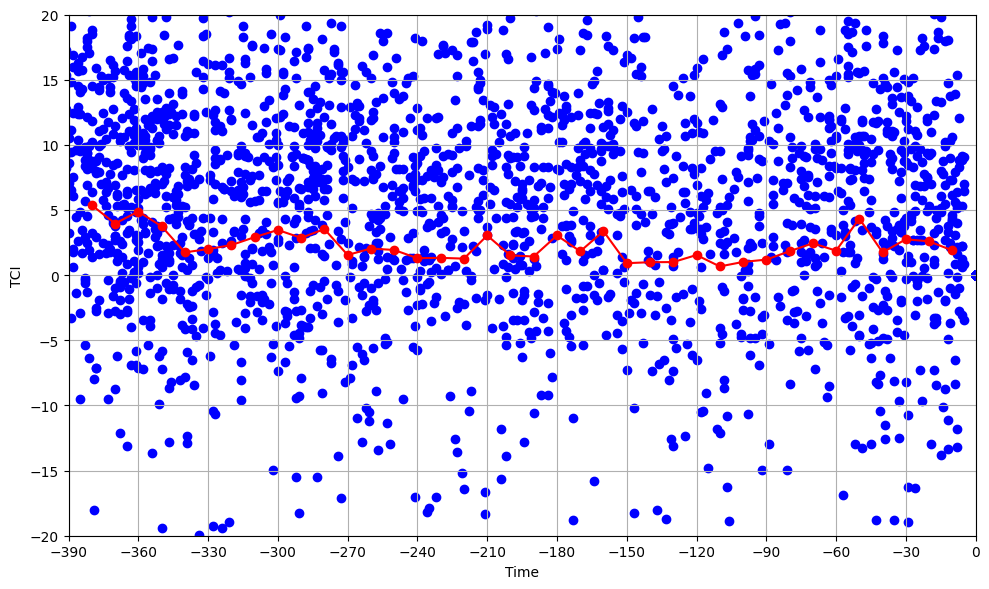
\includegraphics[width=0.9\textwidth]{images/tci_plot.png}
	\caption{نمودار پراکندگی شاخص دوره انتقال در طول زمان نسبت به زایش}
	\label{fig:tci_trend}
\end{figure}

همان‌گونه که در نمودار قابل مشاهده است، هر نقطه نمایانگر یک گاو منفرد و مقدار شاخص آن پس از زایش است. روند کلی میانگین نیز با خط قرمز مشخص شده است تا تغییرات عمومی را بهتر نمایش دهد. 

در مطالعه‌ی لاکروآ و نوردلوند\cite{lacroix2009} نیز شکلی مشابه برای پایش برنامه‌های مدیریت دوره انتقال ارائه شده است. آن‌ها تاکید دارند که در محاسبه‌ی شاخص دوره انتقال، تمامی گاوهایی که اولین رکورد شیر ثبت‌شده دارند، تا ۳۶۵ روز در نمودار و محاسبات لحاظ می‌شوند، حتی اگر از گله حذف شده یا بیمار بوده باشند. این موضوع اهمیت بررسی دقیق داده‌های انفرادی را به‌ویژه برای شناسایی موارد شکست مدیریتی نشان می‌دهد.

با تحلیل نمودار حاضر، مشخص می‌شود که مقدار شاخص دوره انتقال به‌صورت میانگین در نزدیکی صفر باقی می‌ماند، اما پراکندگی قابل‌توجهی در مقادیر وجود دارد. این تنوع می‌تواند ناشی از تفاوت در وضعیت بدنی گاوها، مدیریت فردی دام، سلامت پستان، تغذیه و یا خطاهای رکوردگیری باشد. همچنین دام‌هایی با مقادیر منفی شدید ممکن است نشان‌دهنده اختلالات جدی در دوره انتقال یا بیماری‌های متابولیکی نظیر کتوز یا ورم پستان باشند. 

با استناد به یافته‌های نوردلوند و همکاران، استفاده از این شاخص می‌تواند ابزاری مؤثر برای پایش مداوم و شناسایی مشکلات مدیریتی در گله باشد، به شرطی که ثبت داده‌ها به‌صورت دقیق و منظم انجام شود \cite{lacroix2009}.


\subsection{هیستوگرام شاخص دوره انتقال برای گاوهای تازه‌زا}

برای بررسی توزیع شاخص دوره انتقال در گله مورد مطالعه، هیستوگرامی از مقادیر شاخص دوره انتقال گاوهای تازه‌زا ترسیم شد (شکل \ref{fig:tci_histogram}). در این نمودار، محور افقی مقادیر شاخص و محور عمودی تعداد گاوهای مربوط به هر بازه را نشان می‌دهد.

\begin{figure}[H]
	\centering
	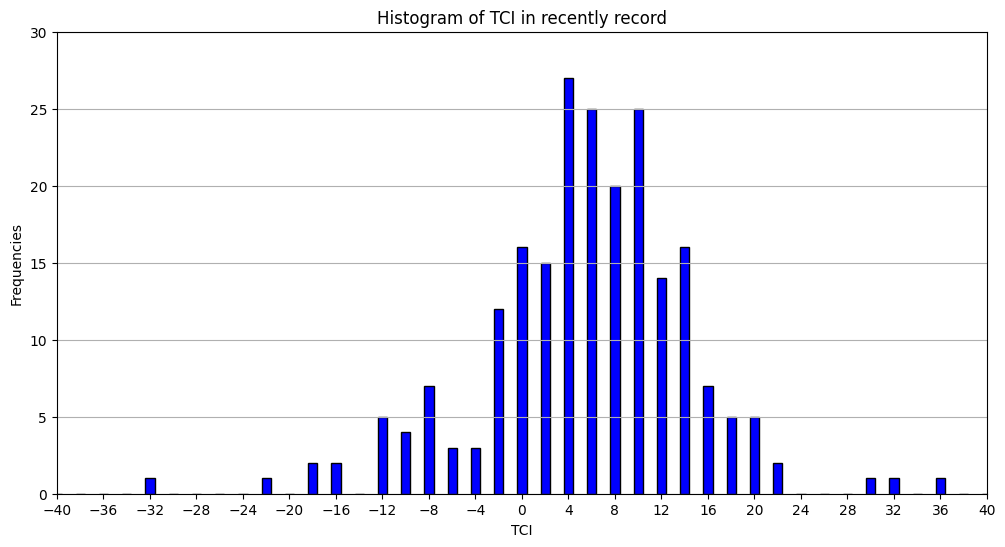
\includegraphics[width=0.9\textwidth]{images/tci_histogram.png}
	\caption{هیستوگرام شاخص دوره انتقال برای گاوهای تازه‌زا}
	\label{fig:tci_histogram}
\end{figure}

همان‌طور که در شکل مشخص است، توزیع داده‌ها نسبتاً نرمال بوده و بیشترین فراوانی مربوط به بازه‌ی ۴ تا ۱۰ است. این موضوع نشان می‌دهد که بیشتر گاوها عملکردی نسبتاً نرمال یا کمی بالاتر از پیش‌بینی در اولین رکورد شیردهی داشته‌اند. مقادیر شاخص نزدیک به صفر نشان‌دهنده آن هستند که عملکرد واقعی دام تقریباً مطابق با مقدار پیش‌بینی‌شده بر اساس داده‌های تاریخی بوده است.

طبق یافته‌های لاکروآ و نوردلوند\cite{lacroix2009}، چون مقدار پیش‌بینی‌شده‌ی اولین رکورد در فرمول شاخص دوره انتقال بر اساس ویژگی‌های مشابه مانند سن، رکورد قبلی، روزهای خشکی و شمارش سلول‌های سوماتیک محاسبه می‌شود، میانگین شاخص دوره انتقال گله معمولاً نزدیک به صفر قرار می‌گیرد.

با این حال، گستره‌ی پراکندگی مقادیر شاخص دوره انتقال می‌تواند تا بیش از ۷۰۰۰ پوند تفاوت را نشان دهد که بیانگر تفاوت چشم‌گیر بین گله‌هایی با مدیریت انتقال موفق و گله‌هایی با مدیریت ضعیف است. در این راستا، ارائه‌ی حدود صدک دهم، میانگین، و صدک نودم به‌عنوان معیارهایی برای مقایسه عملکرد گله‌ها پیشنهاد شده است. چنین اطلاعاتی می‌تواند نه‌تنها برای پژوهشگران، بلکه برای دامداران نیز ابزار مهمی در جهت اصلاح و بهبود برنامه‌های مدیریت دوره انتقال باشد.

با توجه به نمودار حاضر، می‌توان نتیجه گرفت که وضعیت کلی گله در حد نرمال یا نسبتاً مثبت ارزیابی می‌شود، اما وجود تعداد قابل‌توجهی از دام‌ها با مقادیر شاخص دوره انتقال منفی هشدارهایی درباره کیفیت دوره انتقال برخی از گاوها به همراه دارد و می‌تواند انگیزه‌ای برای بررسی دقیق‌تر شرایط مدیریتی، تغذیه‌ای و سلامت گاوهای خاص باشد.

\subsection{روند تغییرات نسبت چربی به پروتئین}

یکی از شاخص‌های مهم در ارزیابی وضعیت متابولیکی گاوهای شیری در اوایل شیردهی، نسبت چربی به پروتئین شیر است. نسبت بالاتر از \num{1.4} معمولاً به‌عنوان نشانه‌ای از بروز کتوز تحت‌کلینیکی در نظر گرفته می‌شود. شکل \ref{fig:fat_protein_ratio} روند تغییرات این نسبت را در طول ماه‌های مختلف رکوردگیری نشان می‌دهد.

\begin{figure}[H]
	\centering
	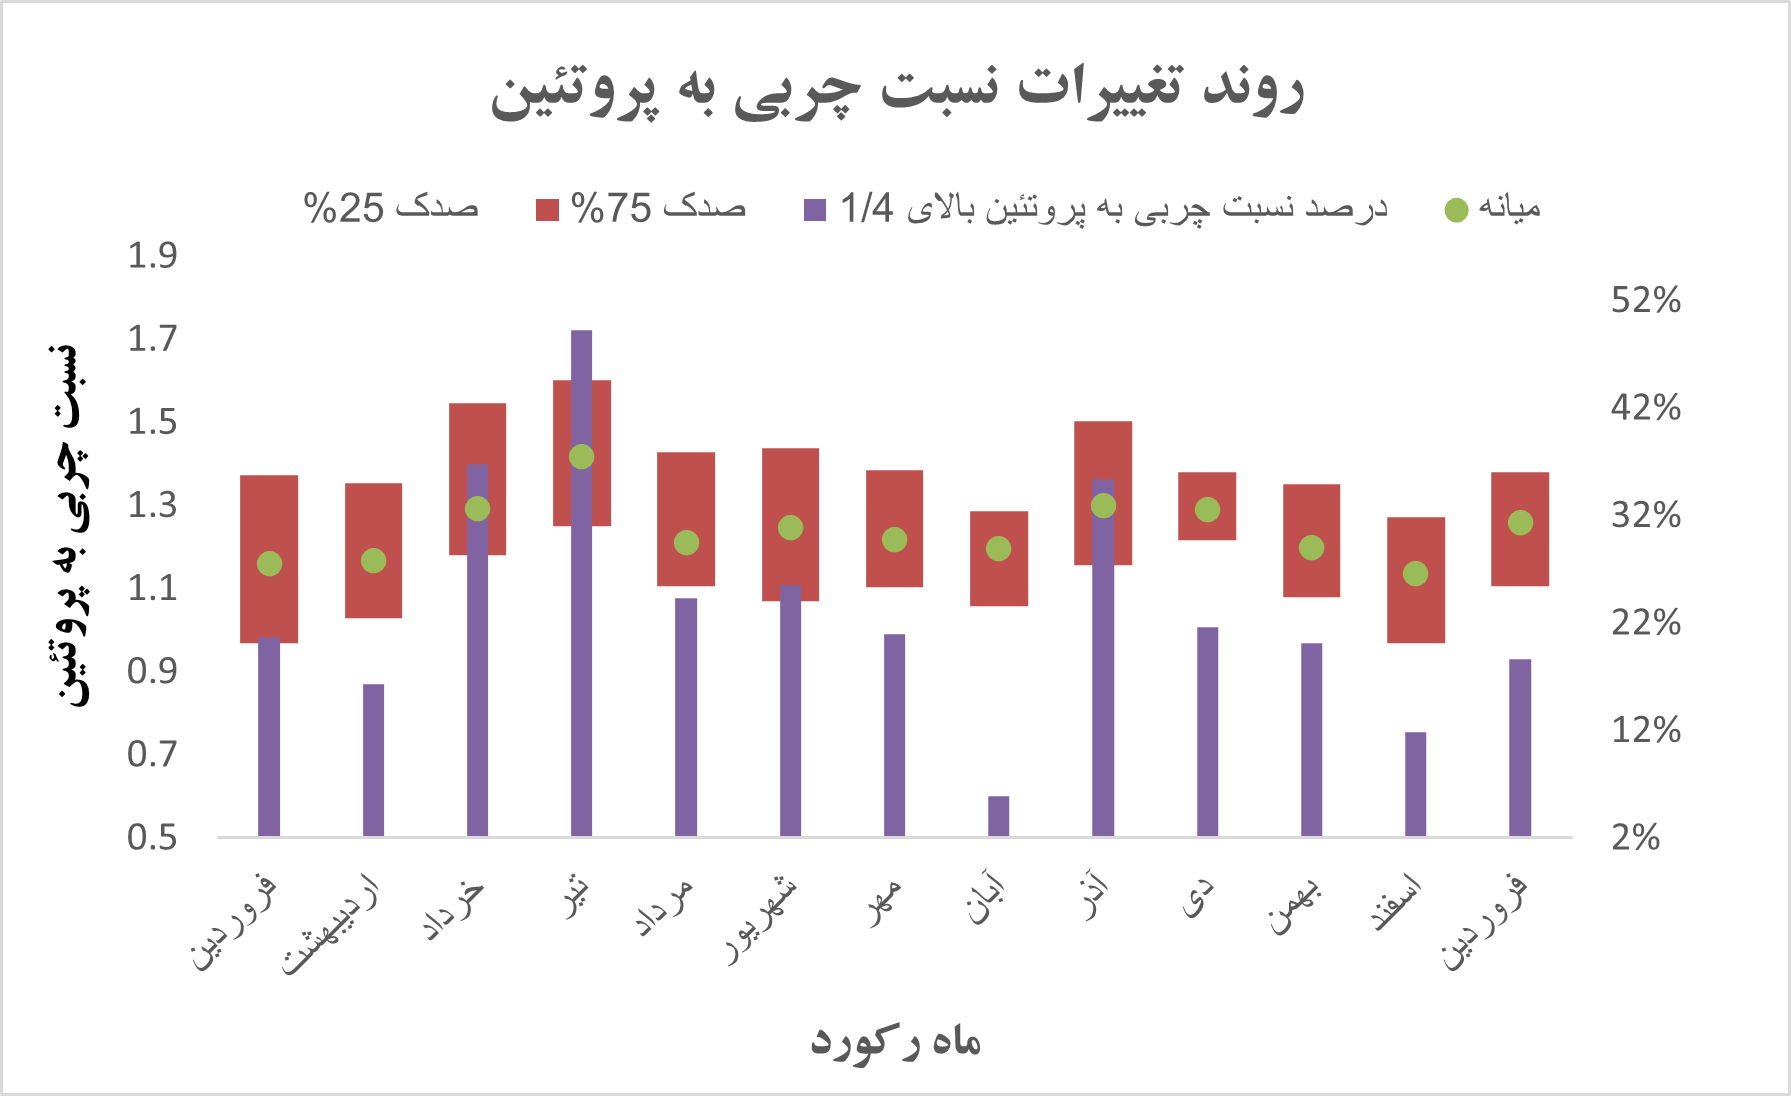
\includegraphics[width=0.9\textwidth]{images/fat_pro.png}
	\caption{روند تغییرات نسبت چربی به پروتئین در طول ماه‌های مختلف}
	\label{fig:fat_protein_ratio}
\end{figure}

در این نمودار، هر ستون شامل اطلاعات مربوط به میانه، صدک ۲۵ و ۷۵، و درصد گاوهایی با نسبت چربی به پروتئین بالاتر از \num{1.4} است:

\begin{itemize}
	\item در ماه‌های خرداد و تیر، نسبت میانه‌ی چربی به پروتئین به بیش از \num{1.4} نزدیک می‌شود که می‌تواند نشان‌دهنده افزایش خطر بروز کتوز در این ماه‌ها باشد.
	\item بیشترین درصد گاوها با نسبت بالاتر از \num{1.4} در همین دو ماه دیده می‌شود (ستون‌های بنفش بلندتر)، که می‌تواند ناشی از استرس گرمایی و تغییرات جیره غذایی در فصل گرم سال باشد.
	\item در مقابل، در ماه‌های آبان، اسفند و اردیبهشت، درصد گاوهایی با نسبت بالا کاهش یافته و میانه نسبت در حد نرمال (حدود \num{1.1} تا \num{1.2}) قرار دارد، که نشان‌دهنده شرایط متابولیکی پایدارتر در این ماه‌ها است.
	\item در بیشتر ماه‌ها، فاصله بین صدک ۲۵ تا ۷۵ گسترده است که نشان می‌دهد تنوع بین گاوها از نظر متابولیسم قابل توجه است و ممکن است نیاز به بررسی‌های مدیریتی انفرادی وجود داشته باشد.
\end{itemize}

با توجه به نقش این شاخص در تشخیص اختلالات متابولیکی، پایش مستمر آن در طول سال می‌تواند به عنوان یک ابزار غربالگری مؤثر برای مدیریت پیشگیرانه سلامت گله در نظر گرفته شود. مقایسه نتایج بین ماه‌های مختلف همچنین می‌تواند به شناسایی الگوهای فصلی در بروز کتوز کمک کند.


\subsection{تعداد ریزش داده خام}

در این بخش، وضعیت حذف داده‌ها در متغیرهای کلیدی برای هر ماه رکورد نمایش داده شده است. جدول \ref{tab:missing_data_months} اطلاعات مربوط به ریزش در هر مرحله پردازش داده برای متغیرهایی مانند شیر ۳۰۵ روزه، مقدار شیر، روزهای شیردهی، طول آبستنی و طول خشکی را نشان می‌دهد.

\begin{table}[H]
	\centering
	\caption{تعداد ریزش داده‌ها به ازای متغیرهای کلیدی در هر ماه رکورد}
	\rowcolors{2}{customblue!30}{white}
	\renewcommand{\arraystretch}{1.3}
	\begin{tabular}{
			 >{\centering\arraybackslash}m{2.8cm} 
			 >{\centering\arraybackslash}m{1.8cm} 
			 >{\centering\arraybackslash}m{1.8cm} 
			 >{\centering\arraybackslash}m{1.8cm} 
			 >{\centering\arraybackslash}m{1.8cm} 
			 >{\centering\arraybackslash}m{1.8cm} 
			 >{\centering\arraybackslash}m{1.8cm} 
		}
		\toprule
		\textbf{ماه رکورد}
		& \textbf{تعداد کل داده‌ها}
		& \textbf{شیر ۳۰۵ روزه}
		& \textbf{مقدار شیر}
		& \textbf{روزهای شیردهی}
		& \textbf{طول آبستنی}
		& \textbf{طول خشکی} \\
		\midrule
		فروردین     & 279 & 0 & 3 & 0 & 5 & 2 \\
		اردیبهشت    & 271 & 0 & 1 & 0 & 0 & 0 \\
		خرداد       & 168 & 0 & 1 & 0 & 5 & 3 \\
		تیر         & 191 & 0 & 2 & 0 & 4 & 2 \\
		مرداد       & 175 & 0 & 0 & 0 & 2 & 1 \\
		شهریور      & 138 & 0 & 0 & 0 & 1 & 1 \\
		مهر         & 170 & 0 & 1 & 0 & 2 & 1 \\
		آبان        & 122 & 0 & 1 & 0 & 1 & 1 \\
		آذر         & 130 & 1 & 2 & 0 & 3 & 1 \\
		دی          & 136 & 0 & 0 & 0 & 6 & 5 \\
		بهمن        & 137 & 0 & 0 & 0 & 3 & 0 \\
		اسفند       & 173 & 0 & 0 & 0 & 4 & 2 \\
		فروردین (سال بعد) & 224 & 0 & 0 & 0 & 3 & 4 \\
		\bottomrule
	\end{tabular}
	\label{tab:missing_data_months}
\end{table}

\textbf{تحلیل جدول:}

\begin{itemize}
	\item بیشترین ریزش مربوط به متغیر \textbf{طول آبستنی} در ماه دی است (۶ مورد)، که ممکن است ناشی از ثبت ناقص اطلاعات آبستنی در آن دوره باشد.
	\item در ماه آذر، داده‌ها از نظر شیر ۳۰۵ روزه و مقدار شیر نیز دچار حذف شده‌اند، که اهمیت کنترل کیفیت ثبت در آن ماه را نشان می‌دهد.
	\item به‌طور کلی، تعداد کل داده‌ها در ماه‌های فروردین، اردیبهشت و تیر بالاتر است که به احتمال زیاد به‌دلیل تراکم زایش‌ها در فصل بهار است.
	\item در بیشتر ماه‌ها، تعداد داده‌های حذف‌شده نسبتاً پایین است که نشان‌دهنده کیفیت قابل قبول داده‌های خام است.
\end{itemize}


\subsection{گاو‌های تازه‌زا با شاخص دوره انتقال کمتر از ۸-}

یکی از مهم‌ترین شاخص‌ها در بررسی عملکرد متابولیکی گاوهای تازه‌زا، شاخص دوره انتقال است. مقادیر منفی زیاد این شاخص می‌تواند بیانگر وجود مشکل در سلامت متابولیکی یا مدیریتی گاوها باشد. در جدول \ref{tab:low_tci_cows}، فهرستی از گاوهایی که مقدار شاخص دوره انتقال آن‌ها کمتر از \num{8}- بوده، ارائه شده است. این جدول شامل اطلاعاتی درباره شماره بدن، دوره شیردهی، روزهای شیردهی، مقدار شاخص دوره انتقال، نسبت چربی به پروتئین، و وضعیت سلامت پستان گاو است.

\begin{table}[H]
	\centering
	\caption{گاوهای تازه‌زا با شاخص دوره انتقال کمتر از \num{8}-}
	\rowcolors{2}{customblue!30}{white}
	\renewcommand{\arraystretch}{1.3}
	\begin{tabular}{
			 >{\centering\arraybackslash}m{2.8cm}
			 >{\centering\arraybackslash}m{1.8cm}
			 >{\centering\arraybackslash}m{1.8cm}
			 >{\centering\arraybackslash}m{2.2cm}
			 >{\centering\arraybackslash}m{2.8cm}
			 >{\centering\arraybackslash}m{2.5cm} 
		}
		\toprule
		\textbf{شماره بدن}
		& \textbf{دوره شیردهی}
		& \textbf{روزهای شیردهی}
		& \textbf{شاخص دوره انتقال}
		& \textbf{نسبت چربی به پروتئین}
		& \textbf{سلامت پستان} \\
		\midrule
		\num{96026} & \num{5} & \num{33} & \num{12.50}- & \num{1.24} & غیر عفونی \\
		\num{96317} & \num{5} & \num{8}  & \num{11.80}- & —         & — \\
		\num{96418} & \num{5} & \num{33} & \num{9.69}-  & \num{0.92} & عفونت جدید \\
		\num{96945} & \num{5} & \num{19} & \num{12.99}- & \num{1.25} & عفونت جدید \\
		\num{36261} & \num{4} & \num{9}  & \num{8.36}-  & \num{1.28} & غیر عفونی \\
		\num{97157} & \num{4} & \num{12} & \num{13.31}- & \num{1.42} & غیر عفونی \\
		\num{97634} & \num{4} & \num{29} & \num{10.72}- & \num{1.48} & عفونت جدید \\
		\num{97834} & \num{4} & \num{35} & \num{18.80}- & —         & — \\
		\num{97849} & \num{4} & \num{15} & \num{13.82}- & \num{1.03} & غیر عفونی \\
		\num{37145} & \num{4} & \num{13} & \num{32.00}- & —         & — \\
		\num{98648} & \num{3} & \num{13} & \num{8.70}-  & \num{1.08} & غیر عفونی \\
		\num{98657} & \num{3} & \num{29} & \num{16.22}- & —         & — \\
		\num{98690} & \num{3} & \num{8}  & \num{13.21}- & —         & — \\
		\num{98854} & \num{3} & \num{30} & \num{8.19}-  & \num{1.10} & غیر عفونی \\
		\num{98969} & \num{3} & \num{17} & \num{8.46}-  & \num{1.34} & عفونت مزمن \\
		\num{38050} & \num{3} & \num{35} & \num{8.16}-  & \num{1.09} & غیر عفونی \\
		\num{38098} & \num{3} & \num{23} & \num{9.63}-  & \num{1.65} & غیر عفونی \\
		\num{38134} & \num{3} & \num{14} & \num{23.75}- & —         & — \\
		\num{99420} & \num{2} & \num{29} & \num{18.95}- & —         & — \\
		\num{99773} & \num{2} & \num{26} & \num{16.34}- & —         & — \\
		\num{99896} & \num{2} & \num{14} & \num{10.11}- & \num{1.33} & غیر عفونی \\
		\num{39252} & \num{2} & \num{12} & \num{11.12}- & —         & — \\
		\bottomrule
	\end{tabular}
	\label{tab:low_tci_cows}
\end{table}

\textbf{تحلیل جدول:}

\begin{itemize}
	\item دام‌هایی با شاخص دوره انتقال بسیار پایین (کمتر از \num{10}-) معمولاً در یکی از شرایط زیر قرار دارند: کاهش شدید شیر در اولین آزمون، وضعیت متابولیکی نامناسب، یا مشکلاتی مانند کتوز یا عفونت پستان.
	\item برخی از گاوهایی که نسبت چربی به پروتئین بالای \num{1.4} داشته‌اند (مانند شماره‌های \num{97634} و \num{97157})، احتمالاً دچار کتوز تحت‌کلینیکی شده‌اند.
	\item درصد قابل توجهی از رکوردها (بیش از \num{30}\%) فاقد اطلاعات نسبت چربی به پروتئین یا سلامت پستان هستند، که این موضوع اهمیت کامل‌بودن داده‌ها در ارزیابی دقیق را نشان می‌دهد.
	\item برخی از موارد، نظیر گاو شماره \num{37145}، دارای شاخص دوره انتقال بسیار منفی (بیش از \num{30}-) بوده‌اند که نیاز به بررسی خاص در مورد عوامل مدیریتی یا بیماری دارد.
\end{itemize}



\section[پیش پردازش داده‌ها]{پیش‌پردازش داده‌ها\LTRfootnote{Data Preprocessing}}

در این بخش، مراحل آماده‌سازی و پاک‌سازی داده‌ها برای مدل‌سازی ارائه می‌شود. ابتدا ساختار کلی مجموعه‌داده توصیف می‌گردد، سپس روش‌های مقابله با مقادیر گمشده، استانداردسازی متغیرها، و تقسیم‌بندی داده‌ها شرح داده شده و در پایان، توزیع آماری متغیرها و ماتریس همبستگی میان آن‌ها تحلیل می‌شود.

\subsection[مجموعه داده]{توصیف مجموعه‌داده\LTRfootnote{Data Set}}

مجموعه‌داده مورد استفاده شامل رکوردهایی از دام‌های موجود در 99 دامداری‌ در سراسر کشور است. این داده‌ها از روی نرم‌افزار سَس\LTRfootnote{SAS} استخراج و در قالب فایل اکسل دریافت شده‌اند. ستون‌های اصلی این مجموعه‌داده به شرح زیر است:

\begin{itemize}
	\item \textbf{گله\LTRfootnote{Hrd}}: شماره گله دام.
	\item \textbf{دوره‌شیردهی\LTRfootnote{milkperiod}}: دوره شیردهی (شکم اول، دوم و ...).
	\item \textbf{سال‌زایش\LTRfootnote{zdate}}: سال زایش دام.
	\item \textbf{ماه‌زایش\LTRfootnote{zdate\_month}}: ماه زایش دام.
	\item \textbf{اولین رکورد شیر\LTRfootnote{firstmilk}}: مقدار شیر ثبت‌شده در اولین رکورد پس از زایمان (متغیر هدف).
	\item \textbf{روز رکورد گیری اولین رکورد شیر\LTRfootnote{firstmilkdays}}: روز ثبت اولین رکورد شیر پس از زایمان.
	\item \textbf{طول دوره آبستنی\LTRfootnote{prelendays}}: مدت آبستنی دام (معمولاً ۹ ماه).
	\item \textbf{طول دوره خشکی\LTRfootnote{drylendays}}: تعداد روزهای خشکی پیش از زایمان بعدی. تقریبا ۲ ماه مانده به زایمان بعدی دام را خشک می‌کنند که به آن دوران خشک می گویند. 	 بعد از زایمان حدود ۲ یا ۳ یا ۴ ماه بعد از زایمان آبستن می شود. وقتی آبستن شد، از ۹ ماه که آبستنه، ۷ ماهه که آبستنه خشکش می کنند.
	.
	\item \textbf{طول دوره شیردهی\LTRfootnote{milkdays}}: طول دوره شیردهی که در واقع نقطه مقابل طول دوره خشکی می‌باشد.
	\item \textbf{گروه\LTRfootnote{grp}}: گروه‌بندی ترکیبی بر اساس دروه‌شیردهی، ماه زایش و طول آبستنی.
	\item \textbf{شیر‌تجمعی 305 روز\LTRfootnote{current\_Milk305}}: مقدار شیر تجمعی در ۳۰۵ روز فعلی.
	\item \textbf{شیر‌تجمعی 305 روز گذشته\LTRfootnote{previous\_Milk305}}: مقدار شیر تجمعی در 305 روز دوره قبلی.
	\item \textbf{اولین رکورد شیر دوره قبلی\LTRfootnote{firstmilk\_previous}}: اولین رکورد شیر دوره قبلی.
	\item \textbf{سلول‌های سوماتیک 305 روز\LTRfootnote{SCS\_305}}: تعداد سلول‌های سوماتیک\LTRfootnote{Somatic Cell Score} در شکم قبلی.
\end{itemize}

در پیش‌پردازش اولیه، رکوردهایی که مقدار روز رکورد گیری اولین رکورد شیر کمتر از ۴ داشتند حذف شدند، چرا که شیر اولیه دام (آغوز) در روزهای ابتدایی پس از زایمان از کیفیت متفاوتی برخوردار است و ثبت آن به عنوان مقدار شیر معیار در مدل‌سازی صحیح نیست. محدوده قابل قبول برای این متغیر از روز چهارم تا سی‌ام پس از زایمان در نظر گرفته شد.

از متغیر گروه نیز به دو صورت در مدل‌ها استفاده شد: (۱) استفاده مستقیم از گروه به عنوان متغیر ترکیبی، (۲) استفاده جداگانه از متغیرهای سازنده آن یعنی ماه‌زایش، طول دوره آبستنی و دوره شیردهی. در بخش مدل‌سازی تفاوت عملکرد این دو رویکرد مورد بحث قرار خواهد گرفت.

\subsection{نمایش توزیع متغیرها}

در این بخش، هیستوگرام توزیع هر یک از متغیرهای عددی مجموعه‌داده به صورت جداگانه نمایش داده شده است. این نمودارها به درک بهتر از چولگی\LTRfootnote{Skewness}، نرمال یا غیرنرمال بودن توزیع\LTRfootnote{Normality} و نیز وجود داده‌های پرت کمک می‌کنند.

\vspace{1cm}

\begin{minipage}{0.48\textwidth}
	\begin{figure}[H]
		\centering
		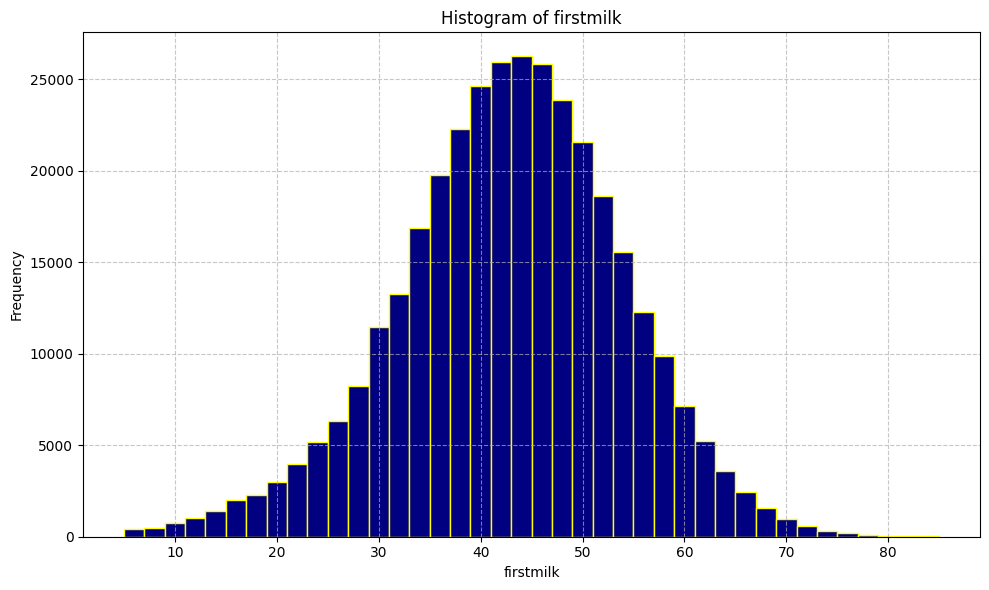
\includegraphics[width=\linewidth]{images/firstmilk.png}
		\caption{هیستوگرام متغیر اولین رکورد شیر}
		\label{fig:firstmilk}
	\end{figure}
\end{minipage}
\hfill
\begin{minipage}{0.48\textwidth}
	\begin{figure}[H]
		\centering
		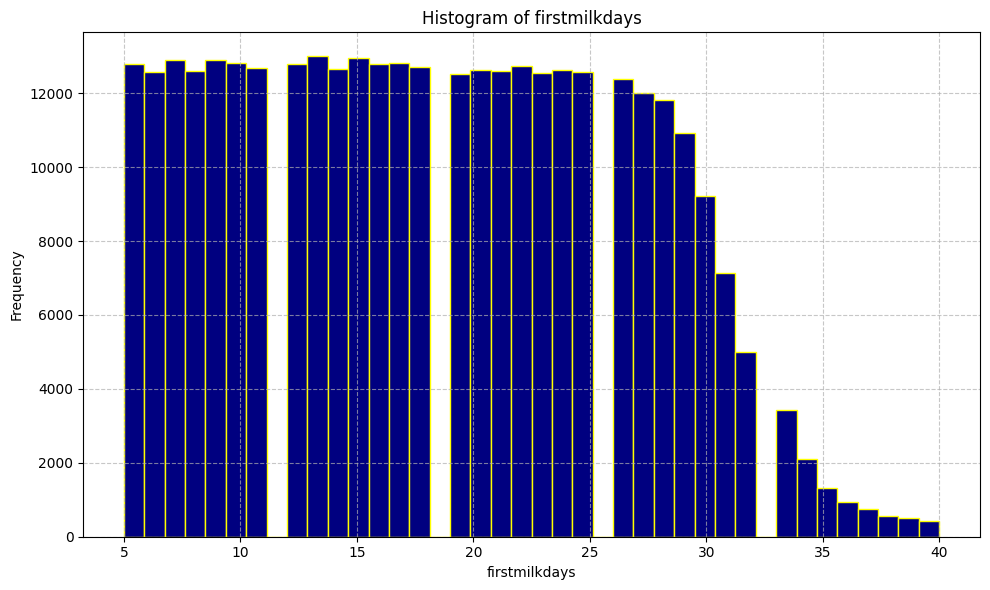
\includegraphics[width=\linewidth]{images/firstmilkdays.png}
		\caption{هیستوگرام متغیر روز رکورد گیری اولین رکورد شیر}
		\label{fig:firstmilkdays}
	\end{figure}
\end{minipage}

\vspace{0.3cm}

\begin{minipage}{0.48\textwidth}
	\begin{figure}[H]
		\centering
		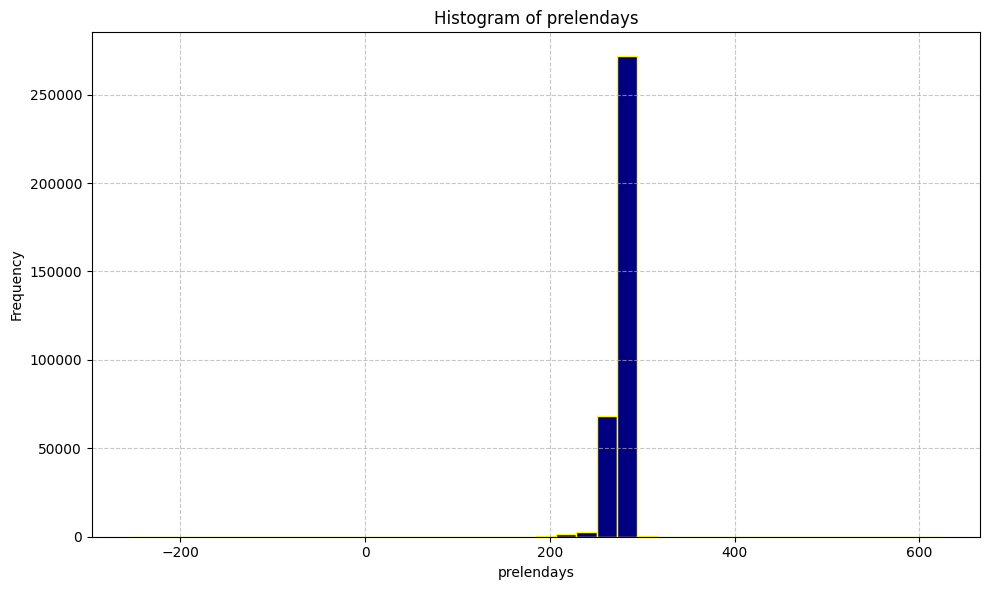
\includegraphics[width=\linewidth]{images/prelendays.png}
		\caption{هیستوگرام متغیر طول دوره آبستنی}
		\label{fig:prelendays}
	\end{figure}
\end{minipage}
\hfill
\begin{minipage}{0.48\textwidth}
	\begin{figure}[H]
		\centering
		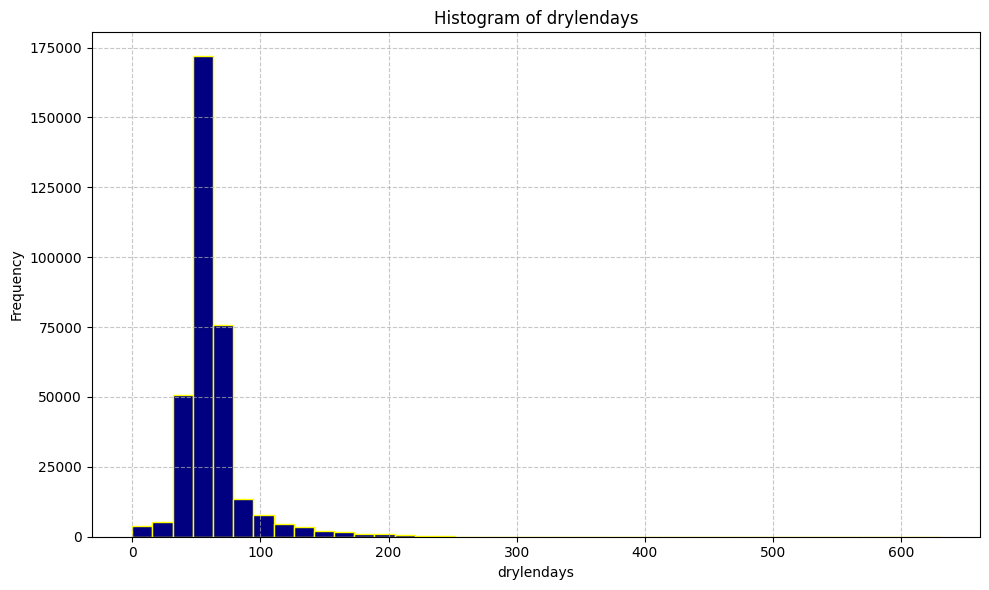
\includegraphics[width=\linewidth]{images/drylendays.png}
		\caption{هیستوگرام متغیر طول دوره خشکی}
		\label{fig:drylendays}
	\end{figure}
\end{minipage}

\vspace{0.3cm}

\begin{minipage}{0.48\textwidth}
	\begin{figure}[H]
		\centering
		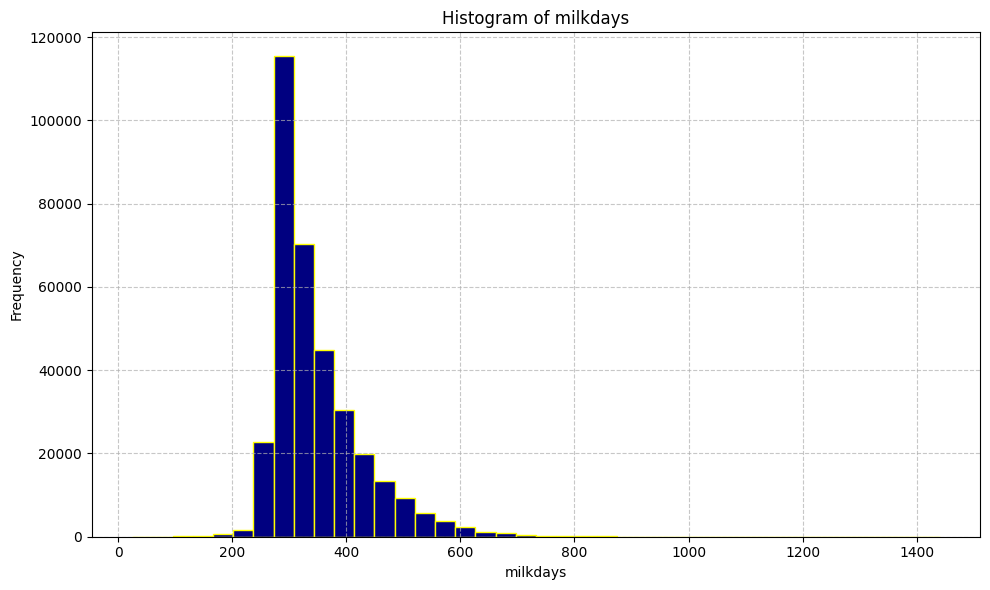
\includegraphics[width=\linewidth]{images/milkdays.png}
		\caption{هیستوگرام متغیر طول دوره شیردهی}
		\label{fig:milkdays}
	\end{figure}
\end{minipage}
\hfill
\begin{minipage}{0.48\textwidth}
	\begin{figure}[H]
		\centering
		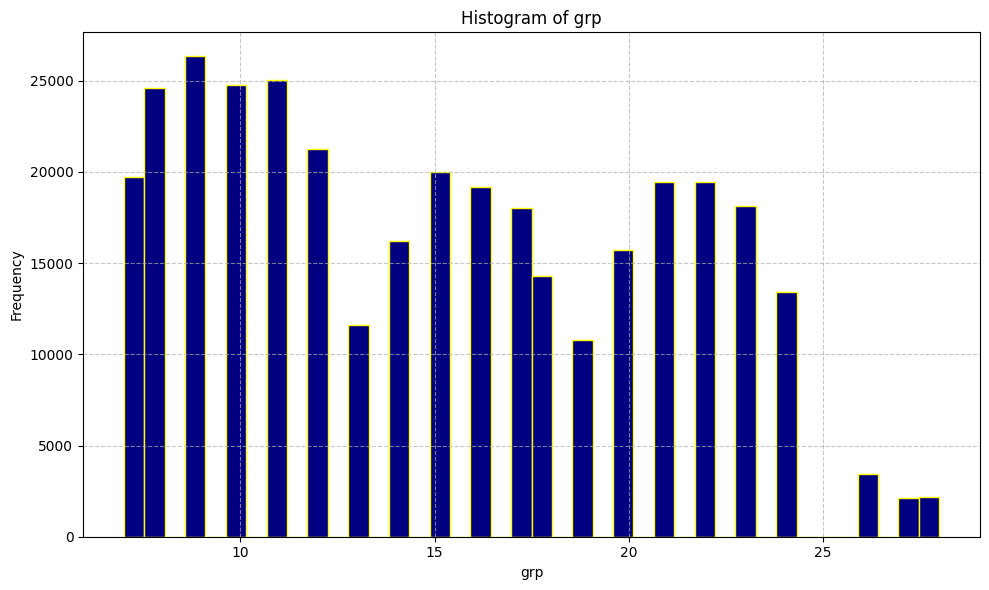
\includegraphics[width=\linewidth]{images/grp.png}
		\caption{هیستوگرام متغیر گروه}
		\label{fig:grp}
	\end{figure}
\end{minipage}

\vspace{0.3cm}

\begin{minipage}{0.48\textwidth}
	\begin{figure}[H]
		\centering
		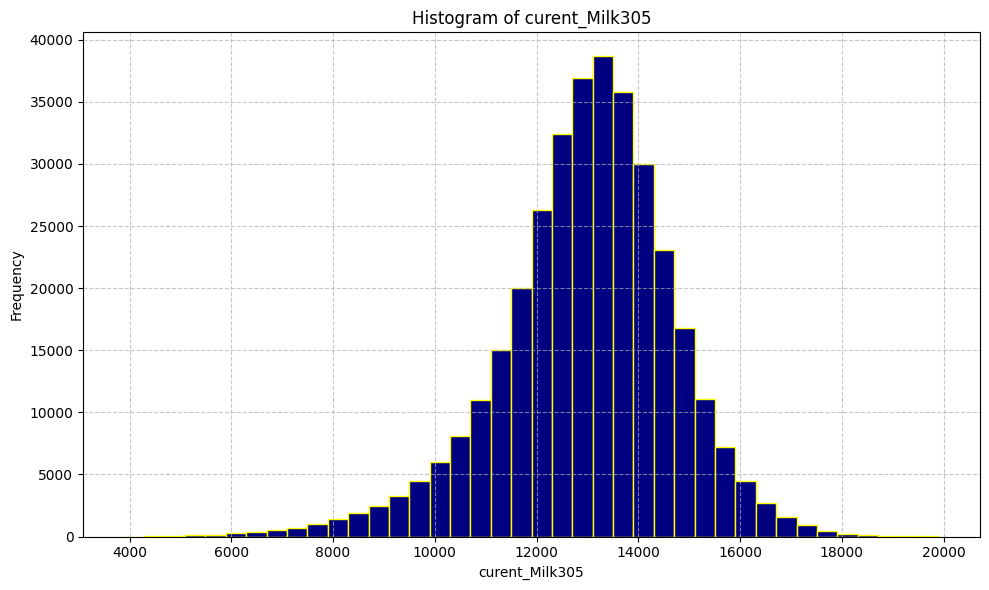
\includegraphics[width=\linewidth]{images/current_Milk305.png}
		\caption{هیستوگرام متغیر شیر‌تجمعی 305 روز}
		\label{fig:curent_Milk305}
	\end{figure}
\end{minipage}
\hfill
\begin{minipage}{0.48\textwidth}
	\begin{figure}[H]
		\centering
		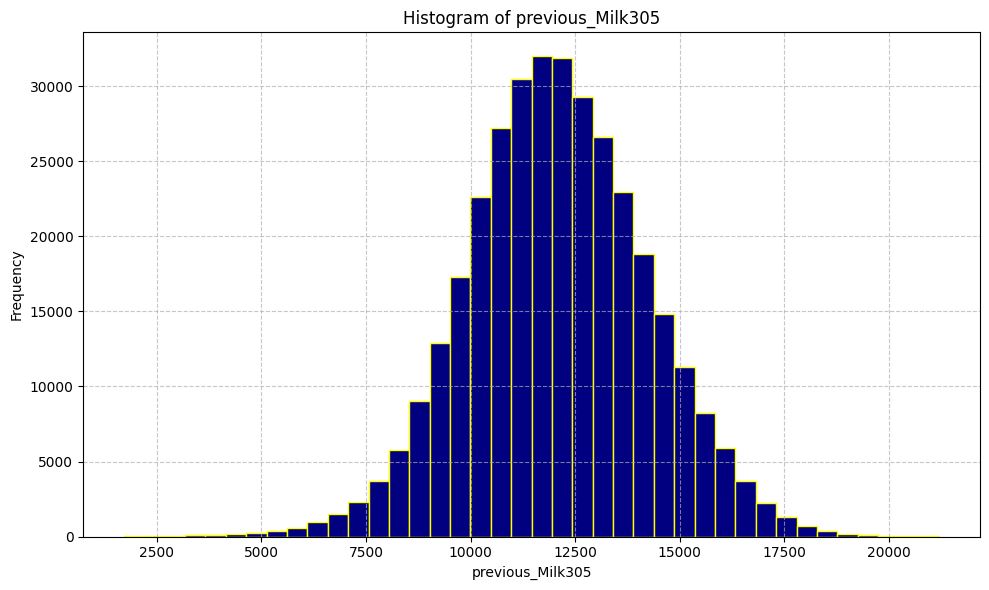
\includegraphics[width=\linewidth]{images/previous_Milk305.png}
		\caption{هیستوگرام متغیر شیر‌تجمعی 305 روز گذشته}
		\label{fig:previous_Milk305}
	\end{figure}
\end{minipage}

\vspace{0.3cm}

\begin{minipage}{0.48\textwidth}
	\begin{figure}[H]
		\centering
		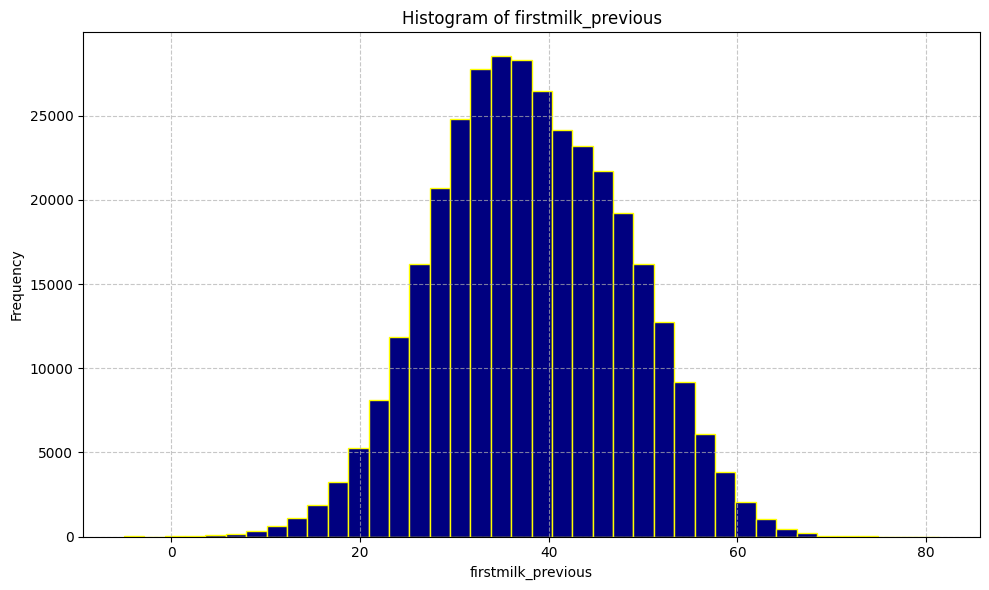
\includegraphics[width=\linewidth]{images/firstmilk_previous.png}
		\caption{هیستوگرام متغیر اولین رکورد شیر دوره قبلی}
		\label{fig:firstmilk_previous}
	\end{figure}
\end{minipage}
\hfill
\begin{minipage}{0.48\textwidth}
	\begin{figure}[H]
		\centering
		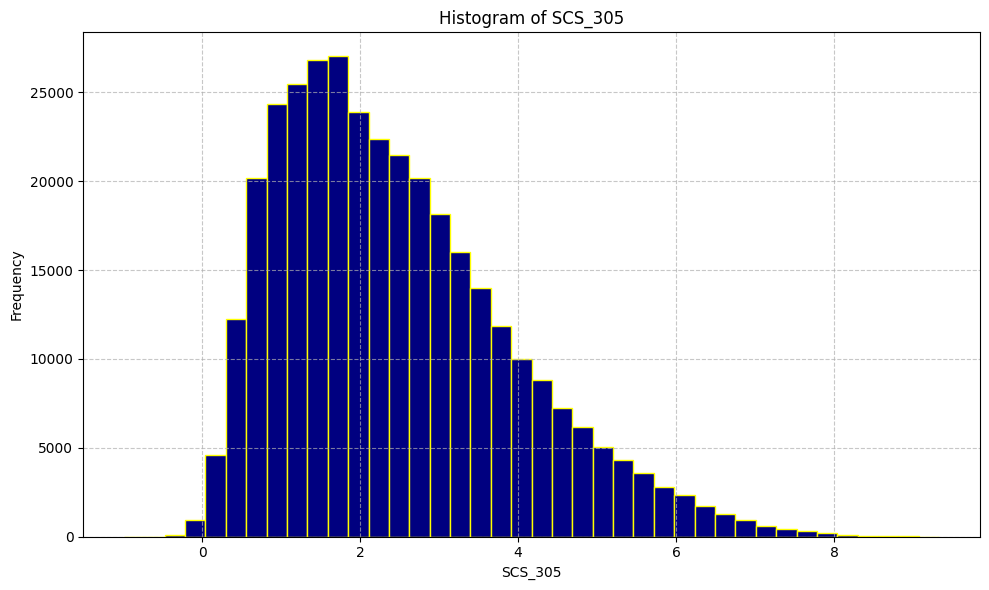
\includegraphics[width=\linewidth]{images/SCS_305.png}
		\caption{هیستوگرام متغیر سلول‌های سوماتیک 305 روز}
		\label{fig:SCS_305}
	\end{figure}
\end{minipage}
\vspace{1cm}


\textbf{تحلیل نمودارها:}
\begin{itemize}
	\item متغیر اولین رکورد شیر دارای توزیعی نسبتاً نرمال و متقارن است که ویژگی مناسبی برای متغیر هدف می‌باشد.
	\item روز رکورد گیری اولین رکورد شیر دارای توزیع یکنواخت در بازه 5 تا 40 روز است که نشان‌دهنده ثبت مناسب و متوازن رکوردها در این بازه است.
	\item طول دوره آبستنی دارای پیک بارزی در محدوده ۲۷۰ تا ۳۰۰ روز است که با طول معمول دوره آبستنی (۹ ماه) مطابقت دارد.
	\item توزیع طول دوره خشکی و روزهای شیردهی هر دو دارای چولگی زیاد هستند که انتخاب میانه برای جایگزینی مقادیر گمشده را توجیه می‌کند.
	\item متغیرهای شیر‌تجمعی 305 روز، شیر‌تجمعی 305 روز گذشته و اولین رکورد شیر دوره قبلی دارای توزیع نسبتاً نرمال هستند که برای مدل‌سازی مطلوب است.
	\item متغیر سلول‌های سوماتیک 305 روز دارای توزیعی چپ‌چوله و تجمع بالا در مقادیر پایین‌تر است که نشان‌دهنده سلامت بالای گله‌ها از نظر سلول‌های سوماتیک است.
\end{itemize}

\subsection{تحلیل ماتریس همبستگی}

شکل \ref{fig:corr_matrix} ماتریس همبستگی بین متغیرهای عددی مجموعه‌داده را نشان می‌دهد. برای محاسبه این همبستگی‌ها از ضریب پیرسون استفاده شده است.

\begin{figure}[H]
	\centering
	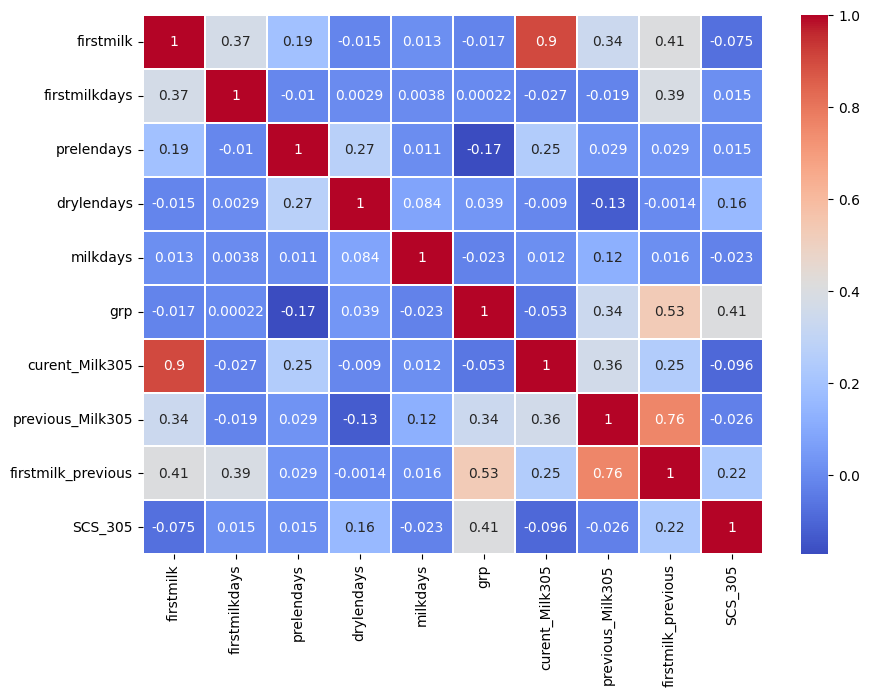
\includegraphics[width=0.85\textwidth]{images/correlation.png}
	\caption{ماتریس همبستگی بین متغیرها}
	\label{fig:corr_matrix}
\end{figure}

\textbf{نکات قابل توجه:}
\begin{itemize}
	\item بالاترین همبستگی با متغیر هدف (اولین رکورد شیر) مربوط به شیر تجمعی 305 روز با مقدار حدود \num{0.9} است. با این حال، از آنجایی که این متغیر از روی اولین رکورد شیر مشتق شده، استفاده از آن در مدل موجب نشت اطلاعات\LTRfootnote{Data Leakage} می‌شود، لذا حذف شد.
	\item متغیرهای اولین رکورد شیر دوره قبلی با متغیر هدف همبستگی مناسبی دارد (حدود \num{0.4}).
	\item همبستگی‌های ضعیف بین متغیرهای دیگر نشان‌دهنده استقلال نسبی آن‌ها و عدم وجود هم‌خطی شدید است.
\end{itemize}


\subsection{مدیریت داده‌های گمشده}

در جدول زیر تعداد مقادیر گمشده در هر ستون از مجموعه‌داده آورده شده است:

\begin{table}[H]
	\centering
	\caption{تعداد داده‌های گمشده در ستون‌ها}
	\rowcolors{2}{customblue!30}{white} % اعمال رنگ مشابه (سورمه‌ای کم‌رنگ برای ردیف‌های زوج)
	\renewcommand{\arraystretch}{1.3} % افزایش فاصله بین ردیف‌ها
	\begin{tabular}{
			>{\centering\arraybackslash}m{4cm} % عرض ستون اول
			>{\centering\arraybackslash}m{3cm} % عرض ستون دوم
		}
		\toprule
		\textbf{نام ستون} & \textbf{تعداد داده گمشده} \\
		\midrule
		milkperiod & \num{0} \\
		zdate & \num{0} \\
		zdate\_month & \num{0} \\
		firstmilk & \num{0} \\
		firstmilkdays & \num{0} \\
		prelendays & \num{0} \\
		drylendays & \num{2059} \\
		milkdays & \num{2059} \\
		previous\_Milk305 & \num{0} \\
		firstmilk\_previous & \num{0} \\
		SCS\_305 & \num{0} \\
		\bottomrule
	\end{tabular}
	\label{tab:missing_data}
\end{table}

برای پر کردن مقادیر گمشده در ستون‌های طول دوره خشکی و روز‌های شیردهی، از مقدار میانه\LTRfootnote{Median} استفاده شد. انتخاب میانه به‌دلیل مقاومت آن در برابر داده‌های پرت و توزیع غیرنرمال این متغیرها انجام شد. مطابق هیستوگرام‌های این متغیرها (شکل \ref{fig:drylendays} و \ref{fig:milkdays}) هر دو دارای توزیعی چولگی‌دار\LTRfootnote{Skewed Distribution} هستند که استفاده از میانگین را نامناسب می‌سازد. در برخی الگوریتم‌هایی که نسبت به داده‌های پرت حساس هستند، این مقادیر گمشده به‌جای جایگزینی حذف شدند.


\subsection{تقسیم‌بندی داده‌ها و نرمال‌سازی}

پس از پاک‌سازی و تکمیل داده‌ها، مجموعه‌داده به سه بخش آموزش (۷۰٪)، اعتبارسنجی (۱۵٪) و آزمون (۱۵٪) تقسیم شد. برای نرمال‌سازی متغیرهای عددی از روش استانداردسازی\LTRfootnote{Standardization} (با استفاده از انحراف معیار و میانگین آموزش) و روش مقیاس‌بندی مقاوم\LTRfootnote{Robust} (با استفاده از میانه و فاصله بین چهارک سوم و اول)استفاده شد. اگرچه جزئیات فنی‌تر این مرحله در بخش مدل‌سازی ارائه خواهد شد، اما در اینجا تأکید می‌شود که نرمال‌سازی تنها بر اساس داده‌های آموزش انجام شده تا از نشت اطلاعات جلوگیری شود.



\section{مدل‌های آموزش داده‌شده}

\subsection{مدل رگرسیون ریج }

یکی از رویکردهای کلیدی در این پژوهش، پیاده‌سازی مدل رگرسیون ریج با استفاده از الگوریتم گرادیان نزولی به صورت دستی بود. این مدل با افزودن جملهٔ منظم‌سازی \textit{\lr{L2}} به تابع هزینه، امکان کنترل پیچیدگی مدل و کاهش بیش‌برازش را فراهم می‌سازد. پیاده‌سازی این مدل به صورت سفارشی انجام شد تا علاوه بر انعطاف در تغییرات، امکان بررسی بهتر جزئیات یادگیری فراهم گردد.

\subsubsection{آماده‌سازی داده‌ها}

برای آموزش مدل، داده‌ها شامل مجموعه‌ای از ویژگی‌های عددی بودند که در جدول \ref{tab:ridge_features} آمده‌اند. متغیر هدف، مقدار اولین رکورد شیر\LTRfootnote{firstmilk} است که بیانگر میزان شیر تولیدشده در نخستین روز از دورهٔ شیردهی جدید دام است.

\begin{table}[H]
	\centering
	\caption{ویژگی‌های استفاده‌شده در مدل رگرسیون ریج}
	\rowcolors{2}{customblue!30}{}
	\renewcommand{\arraystretch}{1.3}
	\begin{tabular}{
			>{\centering\arraybackslash}m{10cm}
		}
		\toprule
		\textbf{ویژگی‌های عددی مورد استفاده} \\
		\midrule
		milkperiod، zdate، zdate\_month، firstmilkdays، prelendays، drylendays، milkdays، previous\_Milk305، firstmilk\_previous، SCS\_305 \\
		\bottomrule
	\end{tabular}
	\label{tab:ridge_features}
\end{table}

برای پر کردن داده‌های گمشده در ستون‌های طول دوره خشکی\LTRfootnote{drylendays} و روز‌های شیردهی\LTRfootnote{milkdays}، از میانه‌ مقادیر آن‌ها استفاده شد(به دلایلی که در بخش قبلی توضیح داده شد). سپس، داده‌ها به سه بخش آموزش (70\%)، اعتبارسنجی (15\%) و آزمون (15\%) تقسیم گردیدند. مجموعه آموزش و اعتبارسنجی برای فرآیند آموزش و تنظیم پارامتر استفاده شده و ارزیابی نهایی فقط بر روی مجموعه آزمون صورت گرفت.

\subsubsection{مقیاس‌بندی ویژگی‌ها}

با توجه به حساسیت الگوریتم گرادیان نزولی به مقیاس ویژگی‌ها، مقادیر عددی ویژگی‌ها به کمک روش استانداردسازی\LTRfootnote{StandardScaler} مقیاس‌بندی شدند. برای جلوگیری از نشت داده، مقیاس‌سازی فقط با استفاده از داده‌های آموزش انجام شده و سپس همان مقیاس روی داده‌های اعتبارسنجی و آزمون اعمال شد.

\subsubsection{آموزش مدل اولیه}

در گام نخست، مدل با مقدار اولیه‌ای از پارامترها آموزش داده شد: نرخ یادگیری\LTRfootnote{Learning rate} \texttt{\lr{۰/۰۱}}، تعداد تکرار\LTRfootnote{Epoch}  \texttt{\lr{۱۰۰۰}} و مقدار منظم‌سازی\LTRfootnote{L2\_lambda}  \texttt{\lr{۰/۱}}. آموزش مدل بر روی داده‌های آموزش انجام شد و عملکرد آن روی مجموعه آزمون ارزیابی گردید.

\vspace{0.3cm}
\begin{table}[H]
	\centering
	\caption{نتایج ارزیابی مدل اولیه رگرسیون ریج بر روی مجموعه آزمون}
	\rowcolors{2}{customblue!30}{white}
	\renewcommand{\arraystretch}{1.3}
	\begin{tabular}{
			>{\centering\arraybackslash}m{4cm}
			>{\centering\arraybackslash}m{3cm}
		}
		\toprule
		\textbf{معیار ارزیابی} & \textbf{مقدار} \\
		\midrule
		ضریب تعیین\LTRfootnote{R\textsuperscript{2}} & \num{0.3110} \\
		میانگین قدرمطلق خطا\LTRfootnote{MAE} & \num{7.0276} \\
		ریشه میانگین مربع خطا\LTRfootnote{RMSE} & \num{9.2071} \\
		درصد خطای میانگین\LTRfootnote{MPE} & \num{8.0856} - \\
		میانگین قدرمطلق درصد خطای متقارن\LTRfootnote{sMAPE} & \num{17.6840} \\
		انحراف استاندارد نسبی\LTRfootnote{SDR} & \num{0.5169} \\
		\bottomrule
	\end{tabular}
	\label{tab:ridge_gd_initial}
\end{table}
\vspace{0.5cm}

\subsubsection{تنظیم پارامترها با استفاده از اعتبارسنجی}

جهت بهینه‌سازی عملکرد مدل، فرایند جست‌وجوی شبکه‌ای\LTRfootnote{Grid Search} برای تعیین بهترین مقادیر نرخ یادگیری، تعداد تکرار و ضریب منظم‌سازی اجرا شد. مجموعه‌ای از ترکیب‌های زیر برای این منظور مورد بررسی قرار گرفت:

\begin{itemize}
	\item نرخ یادگیری: \texttt{\lr{۰/۰۰۱}}، \texttt{\lr{۰/۰۱}}، \texttt{\lr{۰/۱}}
	\item تعداد تکرار: \texttt{\lr{۵۰۰}}، \texttt{\lr{۱۰۰۰}}، \texttt{\lr{۲۰۰۰}}
	\item ضریب منظم‌سازی: \texttt{\lr{۰/۰۰۱}}، \texttt{\lr{۰/۰۱}}، \texttt{\lr{۰/۱}}
\end{itemize}


هر ترکیب روی مجموعه آموزش آموزش داده شد و عملکرد آن روی مجموعه اعتبارسنجی بر اساس میانگین مربعات خطا\LTRfootnote{MSE} سنجیده شد. بهترین ترکیب به صورت زیر شناسایی شد:

\begin{itemize}
	\item نرخ یادگیری: \texttt{\lr{۰/۱}}
	\item تعداد تکرار: \texttt{\lr{۲۰۰۰}}
	\item ضریب منظم‌سازی: \texttt{\lr{۰/۰۰۱}}
\end{itemize}


\subsubsection{آموزش مدل نهایی و ارزیابی}

مدل نهایی با استفاده از مقادیر بهینهٔ به‌دست‌آمده آموزش داده شد. سپس پیش‌بینی مدل روی داده‌های آزمون انجام شد و نتایج نهایی به‌صورت جدول زیر خلاصه شده‌اند:

\vspace{0.3cm}
\begin{table}[H]
	\centering
	\caption{نتایج ارزیابی مدل نهایی رگرسیون ریج بر روی مجموعه آزمون}
	\rowcolors{2}{customblue!30}{white}
	\renewcommand{\arraystretch}{1.3}
	\begin{tabular}{
			>{\centering\arraybackslash}m{4cm}
			>{\centering\arraybackslash}m{3cm}
		}
		\toprule
		\textbf{معیار ارزیابی} & \textbf{مقدار} \\
		\midrule
		ضریب تعیین & \num{0.3134} \\
		میانگین قدرمطلق خطا & \num{7.0057} \\
		ریشه میانگین مربع خطا & \num{9.1909} \\
		درصد خطای میانگین & \num{7.8779} -\\
		میانگین قدرمطلق درصد خطای متقارن & \num{17.6642} \\
		انحراف استاندارد نسبی & \num{0.5571} \\
		\bottomrule
	\end{tabular}
	\label{tab:ridge_gd_final}
\end{table}
\vspace{0.5cm}





\subsection{مدل جنگل تصادفی}

جنگل تصادفی یکی از الگوریتم‌های قدرتمند در یادگیری ماشین است که با استفاده از مجموعه‌ای از درختان تصمیم‌گیری، پایداری و دقت پیش‌بینی را افزایش می‌دهد. در این پژوهش، مدل‌های مختلفی از جنگل تصادفی مورد استفاده قرار گرفتند که شامل مدل اولیه، مدل بهینه‌شده، مدل با اعتبارسنجی متقاطع، و نسخه‌های مبتنی بر ویژگی گروه\LTRfootnote{grp} بودند.

\subsubsection{ویژگی‌های مورد استفاده}
ویژگی‌هایی که برای توسعه مدل جنگل تصادفی استفاده شده‌اند، به دو دسته کلی تقسیم می‌شوند: مدل‌های بدون استفاده از متغیر گروه و مدل‌هایی که این متغیر را در نظر گرفته‌اند.

\paragraph{مدل‌های بدون ویژگی گروه:}
در این نسخه از مدل، متغیرهای زمانی و رکوردهای تاریخی مرتبط با گاو مورد استفاده قرار گرفته‌اند. جدول \ref{tab:rf_features_nogrp} لیست کامل ویژگی‌های استفاده‌شده در این نسخه را نشان می‌دهد.

\begin{table}[H]
	\centering
	\caption{ویژگی‌های استفاده‌شده در مدل جنگل تصادفی بدون متغیر گروه}
	\rowcolors{2}{customblue!30}{}
	\renewcommand{\arraystretch}{1.3}
	\begin{tabular}{
			>{\centering\arraybackslash}m{14cm}
		}
		\toprule
		\textbf{ویژگی‌های عددی مورد استفاده} \\
		\midrule
		\lr{milkperiod}، \lr{zdate}، \lr{zdate\_month}، \lr{firstmilkdays}، \lr{prelendays}، \lr{drylendays}، \lr{milkdays}، \lr{previous\_Milk305}، \lr{firstmilk\_previous}، \lr{SCS\_305} \\
		\bottomrule
	\end{tabular}
	\label{tab:rf_features_nogrp}
\end{table}


\paragraph{مدل‌های با ویژگی گروه:}
در این نسخه از مدل، ویژگی‌های زمانی حذف شده‌اند و متغیر گروه‌بندی جایگزین آن‌ها شده است. جدول \ref{tab:rf_features_grp} فهرست ویژگی‌های نهایی در این نسخه را نمایش می‌دهد.

\begin{table}[H]
	\centering
	\caption{ویژگی‌های استفاده‌شده در مدل جنگل تصادفی با متغیر گروه}
	\rowcolors{2}{customblue!30}{}
	\renewcommand{\arraystretch}{1.3}
	\begin{tabular}{
			>{\centering\arraybackslash}m{14cm}
		}
		\toprule
		\textbf{ویژگی‌های عددی مورد استفاده} \\
		\midrule
		\lr{firstmilkdays}، \lr{prelendays}، \lr{drylendays}، \lr{milkdays}، \lr{grp}، \lr{previous\_Milk305}، \lr{firstmilk\_previous}، \lr{SCS\_305} \\
		\bottomrule
	\end{tabular}
	\label{tab:rf_features_grp}
\end{table}




\subsubsection{آماده‌سازی داده‌ها}

برای آموزش مدل اولیه، از مجموعه‌ای از ویژگی‌های عددی استفاده شد که در مدل رگرسیون ریج نیز به‌کار رفته بودند. داده‌های گمشده در ستون‌های طول دوره خشکی و روزهای شیردهی با مقدار میانه پر شدند و سپس داده‌ها به نسبت ۷۰٪ آموزش، ۱۵٪ اعتبارسنجی و ۱۵٪ آزمون تقسیم شدند.

\subsubsection{مقیاس‌بندی ویژگی‌ها}

مقیاس‌بندی ویژگی‌ها با استفاده از روش استانداردسازی تنها روی داده‌های آموزش انجام گرفت و سپس همان مقیاس روی داده‌های اعتبارسنجی و آزمون اعمال شد.

\subsubsection{آموزش مدل اولیه}

مدل اولیه جنگل تصادفی با پارامترهای پیش‌فرض روی داده‌های آموزش، آموزش داده شد و نتایج آن روی مجموعه آزمون ارزیابی شد.

\begin{table}[H]
	\centering
	\caption{نتایج ارزیابی مدل اولیه جنگل تصادفی}
	\rowcolors{2}{customblue!30}{white}
	\renewcommand{\arraystretch}{1.3}
	\begin{tabular}{>{\centering\arraybackslash}m{4cm} >{\centering\arraybackslash}m{3cm}}
		\toprule
		\textbf{معیار ارزیابی} & \textbf{مقدار} \\
		\midrule
		ضریب تعیین & \num{0.348} \\
		میانگین قدرمطلق خطا & \num{6.829} \\
		ریشه میانگین مربع خطا & \num{8.958} \\
		درصد خطای میانگین & \num{6.936} - \\
		میانگین قدرمطلق درصد خطای متقارن & \num{17.223} \\
		انحراف استاندارد نسبی & \num{0.611} \\
		\bottomrule
	\end{tabular}
	\label{tab:rf_initial}
\end{table}

\subsubsection{تنظیم پارامترها با استفاده از جست‌وجوی شبکه‌ای}

برای بهینه‌سازی مدل، از روش جست‌وجوی شبکه‌ای با اعتبارسنجی پنج‌تایی استفاده شد. بهترین ترکیب پارامترها به شرح زیر شناسایی شد:

\begin{itemize}
	\item تعداد درخت‌ها\LTRfootnote{n\_estimators}: \num{100}
	\item عمق بیشینه درخت‌ها\LTRfootnote{max\_depth}: \num{20}
	\item حداقل نمونه برای تقسیم\LTRfootnote{min\_samples\_split}: \num{10}
	\item حداقل نمونه در برگ\LTRfootnote{min\_samples\_leaf}: \num{4}
\end{itemize}

\subsubsection{آموزش مدل نهایی و ارزیابی}

مدل نهایی با استفاده از مقادیر بهینه آموزش داده شد و نتایج آن بر روی مجموعه آزمون به شرح زیر است:

\begin{table}[H]
	\centering
	\caption{نتایج ارزیابی مدل نهایی جنگل تصادفی}
	\rowcolors{2}{customblue!30}{white}
	\renewcommand{\arraystretch}{1.3}
	\begin{tabular}{>{\centering\arraybackslash}m{4cm} >{\centering\arraybackslash}m{3cm}}
		\toprule
		\textbf{معیار ارزیابی} & \textbf{مقدار} \\
		\midrule
		ضریب تعیین & \num{0.358} \\
		میانگین قدرمطلق خطا & \num{6.759} \\
		ریشه میانگین مربع خطا & \num{8.891} \\
		درصد خطای میانگین & \num{7.316} - \\
		میانگین قدرمطلق درصد خطای متقارن & \num{17.055} \\
		انحراف استاندارد نسبی & \num{0.603} \\
		\bottomrule
	\end{tabular}
	\label{tab:rf_final}
\end{table}

\subsubsection{اعتبارسنجی متقاطع (با پارامترهای نهایی)}

برای بررسی پایداری مدل و جلوگیری از بیش‌برازش، اعتبارسنجی متقاطع پنج‌تایی اجرا شد. نتایج ارزیابی مدل نهایی با اعتبارسنجی متقاطع در جدول زیر آمده است:

\begin{table}[H]
	\centering
	\caption{ارزیابی نهایی مدل جنگل تصادفی با اعتبارسنجی متقاطع}
	\rowcolors{2}{customblue!30}{white}
	\renewcommand{\arraystretch}{1.3}
	\begin{tabular}{>{\centering\arraybackslash}m{4cm} >{\centering\arraybackslash}m{3cm}}
		\toprule
		\textbf{معیار ارزیابی} & \textbf{مقدار} \\
		\midrule
		ضریب تعیین & \num{0.353} \\
		میانگین قدرمطلق خطا & \num{6.785} \\
		ریشه میانگین مربع خطا & \num{8.925} \\
		درصد خطای میانگین & \num{7.611} - \\
		میانگین قدرمطلق درصد خطای متقارن & \num{17.093} \\
		انحراف استاندارد نسبی & \num{0.574} \\
		\bottomrule
	\end{tabular}
	\label{tab:rf_cv_final}
\end{table}

به‌منظور افزایش دقت ارزیابی مدل و جلوگیری از بیش‌برازش، از روش اعتبارسنجی متقاطع پنج‌تایی برای آموزش مدل جنگل تصادفی استفاده شد. در این روش، داده‌های آموزش به پنج بخش تقسیم شده و مدل در هر تکرار روی چهار بخش آموزش دیده و روی بخش پنجم اعتبارسنجی شده است. در نهایت، مدل نهایی روی کل داده‌های آموزش آموزش داده شده و بر روی مجموعه تست، که در فرآیند آموزش شرکت نداشت، ارزیابی شده است.

در جدول \ref{tab:rf_cv_final} نتایج ارزیابی مدل جنگل تصادفی با استفاده از اعتبارسنجی متقاطع ارائه شده است. مقایسه این نتایج با نتایج مدل نهایی بدون اعتبارسنجی (جدول \ref{tab:rf_final}) نشان می‌دهد که عملکرد مدل در هر دو حالت بسیار نزدیک است. به‌عنوان نمونه، مقدار ضریب تعیین در مدل بدون اعتبارسنجی برابر با \num{0.358} و در مدل اعتبارسنجی‌شده برابر با \num{0.353} است که تفاوت بسیار ناچیزی دارد. همچنین مقادیر معیارهای خطا مانند میانگین قدرمطلق خطا و ریشه میانگین مربع خطا نیز به‌طور مشابه نزدیک‌اند (\num{6.759} در مقابل \num{6.785} برای میانگین قدرمطلق خطا، و \num{8.891} در مقابل \num{8.925} برای ریشه میانگین مربع خطا).

این نزدیکی نتایج نشان‌دهنده آن است که مدل دچار بیش‌برازش نشده و عملکرد آن بر روی داده‌های دیده‌نشده پایدار باقی مانده است. همچنین می‌توان نتیجه گرفت که داده‌های آموزش از تنوع و پوشش مناسبی برخوردار بوده‌اند و مدل توانسته الگوهای موجود را به‌خوبی یاد بگیرد.

بنابراین استفاده از اعتبارسنجی متقاطع ضمن فراهم کردن ارزیابی دقیق‌تر، اطمینان بیشتری نسبت به تعمیم‌پذیری مدل نهایی فراهم کرده است. این روند در مطالعات مشابه نیز به عنوان یک رویه استاندارد در ارزیابی مدل‌های یادگیری ماشین توصیه می‌شود.


\subsubsection{مدل‌های مبتنی بر ویژگی گروه}

برای بررسی تأثیر ویژگی گروه، مدل‌های جدیدی با جایگزینی ویژگی‌های زمانی با گروخ طراحی و ارزیابی شدند.

\paragraph{مدل اولیه با گروه:} نتایج ارزیابی مدل اولیه با استفاده از ویژگی گروه به شرح زیر است:

\begin{table}[H]
	\centering
	\caption{نتایج مدل اولیه جنگل تصادفی با گروه}
	\rowcolors{2}{customblue!30}{white}
	\renewcommand{\arraystretch}{1.3}
	\begin{tabular}{>{\centering\arraybackslash}m{4cm} >{\centering\arraybackslash}m{3cm}}
		\toprule
		\textbf{معیار ارزیابی} & \textbf{مقدار} \\
		\midrule
		ضریب تعیین & \num{0.340} \\
		میانگین قدرمطلق خطا & \num{6.879} \\
		ریشه میانگین مربع خطا & \num{9.011} \\
		درصد خطای میانگین & \num{6.964} - \\
		میانگین قدرمطلق درصد خطای متقارن & \num{17.342} \\
		انحراف استاندارد نسبی & \num{0.614} \\
		\bottomrule
	\end{tabular}
	\label{tab:rf_grp_initial}
\end{table}

\paragraph{مدل بهینه‌شده با گروه:} نتایج حاصل از آموزش مدل بهینه‌شده با استفاده از پارامترهای بهینه‌یافته در جدول زیر آمده است:

\begin{table}[H]
	\centering
	\caption{نتایج مدل نهایی جنگل تصادفی با گروه}
	\rowcolors{2}{customblue!30}{white}
	\renewcommand{\arraystretch}{1.3}
	\begin{tabular}{>{\centering\arraybackslash}m{4cm} >{\centering\arraybackslash}m{3cm}}
		\toprule
		\textbf{معیار ارزیابی} & \textbf{مقدار} \\
		\midrule
		ضریب تعیین & \num{0.351} \\
		میانگین قدرمطلق خطا & \num{6.793} \\
		ریشه میانگین مربع خطا & \num{8.933} \\
		درصد خطای میانگین & \num{7.609} - \\
		میانگین قدرمطلق درصد خطای متقارن & \num{17.112} \\
		انحراف استاندارد نسبی & \num{0.575} \\
		\bottomrule
	\end{tabular}
	\label{tab:rf_grp_final}
\end{table}

\paragraph{اعتبارسنجی متقاطع مدل با گروه:} در نهایت، ارزیابی با اعتبارسنجی متقاطع نیز روی این مدل انجام شد و نتایج آن در جدول زیر ارائه می‌گردد:

\begin{table}[H]
	\centering
	\caption{مدل نهایی جنگل تصادفی با گروه و اعتبارسنجی متقاطع}
	\rowcolors{2}{customblue!30}{white}
	\renewcommand{\arraystretch}{1.3}
	\begin{tabular}{>{\centering\arraybackslash}m{4cm} >{\centering\arraybackslash}m{3cm}}
		\toprule
		\textbf{معیار ارزیابی} & \textbf{مقدار} \\
		\midrule
		ضریب تعیین & \num{0.351} \\
		میانگین قدرمطلق خطا & \num{6.793} \\
		ریشه میانگین مربع خطا & \num{8.933} \\
		درصد خطای میانگین & \num{7.609} - \\
		میانگین قدرمطلق درصد خطای متقارن & \num{17.112} \\
		انحراف استاندارد نسبی & \num{0.575} \\
		\bottomrule
	\end{tabular}
	\label{tab:rf_grp_cv_final}
\end{table}



در این بخش، عملکرد مدل جنگل تصادفی با افزودن ویژگی «گروه» (که دسته‌بندی‌های سنی یا شکم گاو را بازتاب می‌دهد) بررسی شد. هدف از اضافه کردن این متغیر، تقویت توان مدل در درک تفاوت‌های ساختاری میان زیرگروه‌های مختلف گاوها و ارتقای دقت پیش‌بینی بود.

نتایج حاصل از آموزش این مدل در جدول \ref{tab:rf_grp_final} آمده است. همان‌طور که مشاهده می‌شود، شاخص‌های ارزیابی تقریباً مشابه با مدل پایه بدون ویژگی گروه هستند. مقدار ضریب تعیین برابر با \num{0.351} است که تفاوت ناچیزی با مدل پایه دارد. همچنین معیارهای خطا نیز بسیار نزدیک به نتایج پیشین هستند.

جالب آن‌که ارزیابی مدل جنگل تصادفی با گروه، در دو حالت با و بدون اعتبارسنجی متقاطع، نتایج یکسانی داشته است (مطابق جدول \ref{tab:rf_grp_cv_final}). این تکرار دقیق نشان می‌دهد که افزودن ویژگی گروه نه تنها عملکرد مدل را تثبیت کرده، بلکه منجر به همگرایی نتایج در فرآیندهای اعتبارسنجی نیز شده است.

این پایداری در نتایج، حاکی از آن است که افزودن متغیر گروه تأثیر معناداری بر بهبود یا افت عملکرد مدل نداشته، اما ممکن است به درک بهتر الگوهای درون‌گروهی کمک کرده باشد. از سوی دیگر، شباهت شاخص‌های ارزیابی بین نسخه اعتبارسنجی‌شده و بدون اعتبارسنجی، بیانگر آن است که مدل از پایداری خوبی برخوردار بوده و دچار بیش‌برازش نشده است.

در مجموع می‌توان گفت که افزودن ویژگی گروه موجب پیچیدگی یا بهبود محسوسی در مدل نشده است، اما بدون ایجاد اثر منفی، می‌تواند به افزایش قابلیت تفسیرپذیری نتایج در سطوح مدیریتی کمک کند.



\subsection{مدل رگرسیون بردار پشتیبان}

یکی از رویکردهای اصلی در این پژوهش، توسعه مدل رگرسیون بردار پشتیبان با استفاده از هسته‌های مختلف بود. این مدل با بهره‌گیری از الگوریتم بهینه‌سازی مبتنی بر بردارهای پشتیبان، امکان پیش‌بینی مقدار شیر تولیدی را با در نظر گرفتن روابط خطی و غیرخطی بین ویژگی‌ها فراهم می‌کند. 

\subsubsection{آماده‌سازی داده‌ها}

ابتدا، داده‌ها از فایل اکسل بارگذاری شدند. ویژگی‌های عددی مورد استفاده برای آموزش مدل در جدول \ref{tab:svr_features} فهرست شده‌اند. متغیر هدف این مدل، مقدار اولین رکورد شیر (\textit{firstmilk}) است که نشان‌دهنده تولید شیر در نخستین روز دوره شیردهی جدید دام می‌باشد.

\begin{table}[H]
	\centering
	\caption{ویژگی‌های استفاده‌شده در مدل رگرسیون بردار پشتیبان}
	\rowcolors{2}{customblue!30}{}
	\renewcommand{\arraystretch}{1.3}
	\begin{tabular}{
			>{\centering\arraybackslash}m{10cm}
		}
		\toprule
		\textbf{ویژگی‌های عددی مورد استفاده} \\
		\midrule
		\lr{milkperiod}، \lr{zdate}، \lr{zdate\_month}، \lr{firstmilkdays}، \lr{prelendays}، \lr{drylendays}، \lr{milkdays}، \lr{previous\_Milk305}، \lr{firstmilk\_previous}، \lr{SCS\_305} \\
		\bottomrule
	\end{tabular}
	\label{tab:svr_features}
\end{table}

برای مدیریت داده‌های گمشده، ابتدا ستون‌های \textit{drylendays} و \textit{milkdays} که حاوی مقادیر خالی بودند، شناسایی شدند. سپس، این مقادیر با استفاده از میانه همان ستون‌ها پر شدند تا از تأثیر داده‌های پرت در توزیع داده‌ها جلوگیری شود. پس از این مرحله، داده‌ها به سه مجموعه تقسیم شدند: مجموعه آموزش (70\%)، مجموعه اعتبارسنجی (15\%) و مجموعه آزمون (15\%). 

\subsubsection{مقیاس‌بندی ویژگی‌ها}

مقیاس‌بندی ویژگی‌ها با استفاده از روش استانداردسازی تنها روی داده‌های آموزش انجام گرفت و سپس همان مقیاس روی داده‌های اعتبارسنجی و آزمون اعمال شد.

\subsubsection{آموزش مدل‌های با هسته‌های خطی، چندجمله‌ای و شعاعی}

در مرحله اول، مدل رگرسیون بردار پشتیبان با هسته خطی پیاده‌سازی شد. پارامترهای اولیه شامل نرخ منظم‌سازی (\textit{C}) با مقدار پیش‌فرض \texttt{\lr{۰/۱}}، نرخ تلرانس (\textit{epsilon}) با مقدار پیش‌فرض \texttt{\lr{۰/۱}}، و حداکثر تعداد تکرار (\textit{max\_iter}) با مقدار پیش‌فرض \texttt{\lr{۱۰۰۰}} بودند. مدل روی مجموعه آموزش، آموزش داده شد. سپس، پیش‌بینی روی مجموعه آزمون انجام شد و معیارهای ارزیابی محاسبه شدند.

\vspace{0.3cm}
\begin{table}[H]
	\centering
	\caption{نتایج ارزیابی مدل اولیه رگرسیون بردار پشتیبان (هسته خطی) بر روی مجموعه آزمون}
	\rowcolors{2}{customblue!30}{white}
	\renewcommand{\arraystretch}{1.3}
	\begin{tabular}{
			>{\centering\arraybackslash}m{4cm}
			>{\centering\arraybackslash}m{3cm}
		}
		\toprule
		\textbf{معیار ارزیابی} & \textbf{مقدار} \\
		\midrule
		ضریب تعیین & \num{0.307} \\
		میانگین قدرمطلق خطا & \num{6.971} \\
		ریشه میانگین مربع خطا & \num{9.233} \\
		درصد خطای میانگین & \num{9.731} - \\
		میانگین قدرمطلق درصد خطای متقارن & \num{17.584} \\
		انحراف استاندارد نسبی & \num{0.585} \\
		\bottomrule
	\end{tabular}
	\label{tab:svr_initial_linear}
\end{table}
\vspace{0.5cm}

سپس، مدل با هسته چندجمله‌ای و هسته شعاعی با همان پارامترهای پیش‌فرض آموزش داده شد. پیش‌بینی و محاسبه معیارها به‌صورت مشابه انجام شد.

\vspace{0.3cm}
\begin{table}[H]
	\centering
	\caption{نتایج ارزیابی مدل اولیه رگرسیون بردار پشتیبان (هسته چندجمله‌ای) بر روی مجموعه آزمون}
	\rowcolors{2}{customblue!30}{white}
	\renewcommand{\arraystretch}{1.3}
	\begin{tabular}{
			>{\centering\arraybackslash}m{4cm}
			>{\centering\arraybackslash}m{3cm}
		}
		\toprule
		\textbf{معیار ارزیابی} & \textbf{مقدار} \\
		\midrule
		ضریب تعیین & \num{0.265} \\
		میانگین قدرمطلق خطا & \num{7.216} \\
		ریشه میانگین مربع خطا & \num{9.511} \\
		درصد خطای میانگین\ & \num{9.821} - \\
		میانگین قدرمطلق درصد خطای متقارن & \num{18.176} \\
		انحراف استاندارد نسبی & \num{0.555} \\
		\bottomrule
	\end{tabular}
	\label{tab:svr_initial_poly}
\end{table}
\vspace{0.3cm}

\begin{table}[H]
	\centering
	\caption{نتایج ارزیابی مدل اولیه رگرسیون بردار پشتیبان (هسته شعاعی) بر روی مجموعه آزمون}
	\rowcolors{2}{customblue!30}{white}
	\renewcommand{\arraystretch}{1.3}
	\begin{tabular}{
			>{\centering\arraybackslash}m{4cm}
			>{\centering\arraybackslash}m{3cm}
		}
		\toprule
		\textbf{معیار ارزیابی} & \textbf{مقدار} \\
		\midrule
		ضریب تعیین & \num{0.364} \\
		میانگین قدرمطلق خطا & \num{6.638} \\
		ریشه میانگین مربع خطا & \num{8.844} \\
		درصد خطای میانگین & \num{9.238} - \\
		میانگین قدرمطلق درصد خطای متقارن & \num{16.759} \\
		انحراف استاندارد نسبی & \num{0.616} \\
		\bottomrule
	\end{tabular}
	\label{tab:svr_initial_rbf}
\end{table}
\vspace{0.5cm}

\subsubsection[مقاوم]{توسعه مدل با هسته شعاعی و مقیاس‌دهی مقاوم\LTRfootnote{RobustScaler}}

برای بررسی تأثیر روش‌های مختلف مقیاس‌بندی و مدیریت داده‌های گمشده، مدل رگرسیون بردار پشتیبان با هسته شعاعی و استفاده از مقیاس بندی مقاوم توسعه یافت. در این بخش، فرآیند آماده‌سازی، مقیاس‌بندی، و ارزیابی این مدل به‌صورت گام‌به‌گام توضیح داده می‌شود.

\paragraph{آماده‌سازی داده‌ها:}
داده‌ها از فایل اکسل بارگذاری شدند. برخلاف مدل‌های قبلی که داده‌های گمشده با میانه پر می‌شدند، در این مدل، داده‌های حاوی مقادیر گمشده حذف شدند تا مجموعه‌ای بدون داده‌های ناقص ایجاد شود. سپس، ویژگی‌ها و متغیر هدف جدا شدند. داده‌ها به سه مجموعه تقسیم شدند: مجموعه آموزش (70\%)، مجموعه اعتبارسنجی (15\%)، و مجموعه آزمون (15\%). 

\paragraph{مقیاس‌بندی ویژگی‌ها:}
به دلیل حساسیت رگرسیون بردار پشتیبان به مقیاس ویژگی‌ها، از روش مقیاس‌دهی مقاوم استفاده شد که نسبت به داده‌های پرت مقاوم‌تر است. 

\paragraph{آموزش و ارزیابی مدل:}
مدل رگرسیون بردار پشتیبان با هسته شعاعی و پارامترهای پیش‌فرض روی مجموعه آموزش مقیاس‌شده آموزش داده شد. پیش‌بینی روی مجموعه آزمون انجام شد و معیارهای ارزیابی با توابع سفارشی و آماده محاسبه شدند.

\vspace{0.3cm}
\begin{table}[H]
	\centering
	\caption{نتایج ارزیابی مدل رگرسیون بردار پشتیبان (با هسته شعاعی و مقیاس‌بندی مقاوم) بر روی مجموعه آزمون}
	\rowcolors{2}{customblue!30}{white}
	\renewcommand{\arraystretch}{1.3}
	\begin{tabular}{
			>{\centering\arraybackslash}m{4cm}
			>{\centering\arraybackslash}m{3cm}
		}
		\toprule
		\textbf{معیار ارزیابی} & \textbf{مقدار} \\
		\midrule
		ضریب تعیین & \num{0.360} \\
		میانگین قدرمطلق خطا & \num{6.644} \\
		ریشه میانگین مربع خطا & \num{8.861} \\
		درصد خطای میانگین & \num{9.240} - \\
		میانگین قدرمطلق درصد خطای متقارن & \num{16.776} \\
		انحراف استاندارد نسبی & \num{0.617} \\
		\bottomrule
	\end{tabular}
	\label{tab:svr_robust_rbf}
\end{table}
\vspace{0.5cm}


\subsection{مدل افزایش گرادیان افراطی}
یکی از رویکردهای کلیدی در این پژوهش، استفاده از مدل افزایش گرادیان افراطی برای پیش‌بینی مقدار شیر تولیدی بود. این مدل با ترکیب چندین درخت تصمیم به‌صورت ترتیبی، امکان یادگیری دقیق‌تر روابط پیچیده بین ویژگی‌ها را فراهم می‌کند.

\subsubsection{آماده‌سازی داده‌ها}

داده‌ها از فایل اکسل بارگذاری شدند. ویژگی‌های عددی مورد استفاده برای آموزش مدل در جدول \ref{tab:xgboost_features} فهرست شده‌اند. متغیر هدف این مدل، مقدار اولین رکورد شیر (\textit{firstmilk}) است که نشان‌دهنده تولید شیر در نخستین روز دوره شیردهی جدید دام می‌باشد.

\begin{table}[H]
	\centering
	\caption{ویژگی‌های استفاده‌شده در مدل افزایش گرادیان افراطی}
	\rowcolors{2}{customblue!30}{}
	\renewcommand{\arraystretch}{1.3}
	\begin{tabular}{
			>{\centering\arraybackslash}m{10cm}
		}
		\toprule
		\textbf{ویژگی‌های عددی مورد استفاده} \\
		\midrule
		\lr{milkperiod}، \lr{zdate}، \lr{zdate\_month}، \lr{firstmilkdays}، \lr{prelendays}، \lr{drylendays}، \lr{milkdays}، \lr{previous\_Milk305}، \lr{firstmilk\_previous}، \lr{SCS\_305} \\
		\bottomrule
	\end{tabular}
	\label{tab:xgboost_features}
\end{table}

برای مدیریت داده‌های گمشده، ستون‌های \textit{drylendays} و \textit{milkdays} که حاوی مقادیر خالی بودند، با استفاده از میانه همان ستون‌ها پر شدند. سپس، داده‌ها به سه مجموعه تقسیم شدند: مجموعه آموزش (70\%)، مجموعه اعتبارسنجی (15\%) و مجموعه آزمون (15\%).

\subsubsection{مقیاس‌بندی ویژگی‌ها}

مقیاس‌بندی ویژگی‌ها با استفاده از روش استانداردسازی تنها روی داده‌های آموزش انجام گرفت و سپس همان مقیاس روی داده‌های اعتبارسنجی و آزمون اعمال شد.

\subsubsection{آموزش مدل اولیه}

در مرحله اول، مدل افزایش گرادیان افراطی با پارامترهای پیش‌فرض روی مجموعه آموزش آموزش داده شد. سپس، پیش‌بینی روی مجموعه آزمون انجام شد و معیارهای ارزیابی محاسبه شدند.

\vspace{0.3cm}
\begin{table}[H]
	\centering
	\caption{نتایج ارزیابی مدل اولیه افزایش گرادیان افراطی بر روی مجموعه آزمون}
	\rowcolors{2}{customblue!30}{white}
	\renewcommand{\arraystretch}{1.3}
	\begin{tabular}{
			>{\centering\arraybackslash}m{4cm}
			>{\centering\arraybackslash}m{3cm}
		}
		\toprule
		\textbf{معیار ارزیابی} & \textbf{مقدار} \\
		\midrule
		ضریب تعیین & \num{0.367} \\
		میانگین قدرمطلق خطا & \num{6.691} \\
		ریشه میانگین مربع خطا & \num{8.827} \\
		درصد خطای میانگین & \num{7.290} - \\
		میانگین قدرمطلق درصد خطای متقارن & \num{16.906} \\
		انحراف استاندارد نسبی & \num{0.618} \\
		\bottomrule
	\end{tabular}
	\label{tab:xgboost_initial}
\end{table}
\vspace{0.5cm}

تحلیل بیش‌برازش نشان داد که اختلاف ضریب تعیین بین مجموعه‌های آموزش و اعتبارسنجی (\texttt{\lr{۰/۰۶۰۲}}) از آستانه \texttt{\lr{۰/۰۵}} بیشتر است، که می‌تواند نشانه‌ای از بیش‌برازش باشد.

\subsubsection{آموزش مدل بهینه‌شده}

برای بهبود عملکرد مدل، پارامترهای مدل با استفاده از جست‌وجوی شبکه‌ای تنظیم شدند. پارامترهای بهینه‌شده شامل تعداد برآوردگرها (\lr{\textit{n\_estimators} = \num{200}})، عمق حداکثر (\lr{\textit{max\_depth} = \num{5}})، نرخ یادگیری (\lr{\textit{learning\_rate} = \num{0.1}})، وزن حداقل فرزند (\lr{\textit{min\_child\_weight} = \num{5}})، نمونه‌برداری (\lr{\textit{subsample} = \num{0.8}})، و نمونه‌برداری از ستون‌ها (\lr{\textit{colsample\_bytree} = \num{0.7}}) بودند. مدل با این پارامترها روی مجموعه آموزش آموزش داده شد و پیش‌بینی روی مجموعه آزمون انجام شد.

\vspace{0.3cm}
\begin{table}[H]
	\centering
	\caption{نتایج ارزیابی مدل بهینه‌شده افزایش گرادیان افراطی بر روی مجموعه آزمون}
	\rowcolors{2}{customblue!30}{white}
	\renewcommand{\arraystretch}{1.3}
	\begin{tabular}{
			>{\centering\arraybackslash}m{4cm}
			>{\centering\arraybackslash}m{3cm}
		}
		\toprule
		\textbf{معیار ارزیابی} & \textbf{مقدار} \\
		\midrule
		ضریب تعیین & \num{0.373} \\
		میانگین قدرمطلق خطا & \num{6.660} \\
		ریشه میانگین مربع خطا & \num{8.783} \\
		درصد خطای میانگین & \num{7.319} - \\
		میانگین قدرمطلق درصد خطای متقارن & \num{16.822} \\
		انحراف استاندارد نسبی & \num{0.607} \\
		\bottomrule
	\end{tabular}
	\label{tab:xgboost_tuned}
\end{table}
\vspace{0.5cm}

تحلیل بیش‌برازش نشان داد که اختلاف ضریب تعیین بین مجموعه‌های آموزش و اعتبارسنجی (\texttt{\lr{۰/۰۲۵۸}}) کمتر از آستانه \texttt{\lr{۰/۰۵}} است، که نشان‌دهنده عدم وجود بیش‌برازش قابل‌توجه است. تیون کردن مدل با پارامترهای بهینه‌شده باعث شد تا مدل از وضعیت بیش‌برازش خارج شده و پایداری بیشتری پیدا کند. این بهبود با کاهش اختلاف ضریب تعیین از \texttt{\lr{۰/۰۶۰۲}} در مدل اولیه به (texttt{\lr{۰/۰۲۵۸}}) در مدل بهینه‌شده تأیید می‌شود، که نشان‌دهنده تعادل بهتر بین دقت و تعمیم‌پذیری است.


\subsection{مدل تقویت دسته‌ای}

یکی از رویکردهای کلیدی در این پژوهش، استفاده از مدل تقویت دسته‌ای برای پیش‌بینی مقدار شیر تولیدی بود. این مدل با بهره‌گیری از الگوریتم‌های مبتنی بر درخت تصمیم و بهینه‌سازی برای مدیریت داده‌های دسته‌ای، دقت بالایی در پیش‌بینی ارائه می‌دهد.

\subsubsection{آماده‌سازی داده‌ها}

داده‌ها از فایل اکسل بارگذاری شدند. ویژگی‌های عددی و دسته‌ای مورد استفاده برای آموزش مدل در جدول \ref{tab:catboost_features} فهرست شده‌اند. متغیر هدف این مدل، مقدار اولین رکورد شیر (\textit{firstmilk}) است که نشان‌دهنده تولید شیر در نخستین روز دوره شیردهی جدید دام می‌باشد.

\begin{table}[H]
	\centering
	\caption{ویژگی‌های استفاده‌شده در مدل تقویت دسته‌ای}
	\rowcolors{2}{customblue!30}{}
	\renewcommand{\arraystretch}{1.3}
	\begin{tabular}{
			>{\centering\arraybackslash}m{10cm}
		}
		\toprule
		\textbf{ویژگی‌های عددی و دسته‌ای مورد استفاده} \\
		\midrule
		\lr{Hrd}، \lr{milkperiod}، \lr{zdate}، \lr{zdate\_month}، \lr{firstmilkdays}، \lr{prelendays}، \lr{drylendays}، \lr{milkdays}، \lr{grp}، \lr{previous\_Milk305}، \lr{firstmilk\_previous}، \lr{SCS\_305} \\
		\bottomrule
	\end{tabular}
	\label{tab:catboost_features}
\end{table}

برای مدیریت داده‌های گمشده، ردیف‌هایی که مقادیر خالی در ستون‌های \textit{drylendays} و \textit{milkdays} داشتند حذف شدند. همچنین، داده‌های نامعتبر (مثبت نبودن مقادیر) فیلتر شدند. پس از آن، یک ویژگی جدید \textit{is\_abortion} با استفاده از شرط \lr{\textit{prelendays} < 260} ایجاد شد تا نشان‌دهنده وقوع سقط در دام باشد. این ویژگی به این منظور اضافه شد که طول دوره آبستنی کمتر از 260 روز را به‌عنوان نشانه‌ای از سقط جنین در نظر بگیرد، که در این صورت مقدار آن به‌صورت باینری (1 برای سقط و 0 برای عدم سقط) تنظیم می‌شود. ستون دسته‌ای \textit{grp} به‌صورت باینری رمزگذاری شد. داده‌ها به سه مجموعه تقسیم شدند: مجموعه آموزش (70\%)، مجموعه اعتبارسنجی (15\%) و مجموعه آزمون (15\%).

\subsubsection{مقیاس‌بندی ویژگی‌ها}

مقیاس‌بندی ویژگی‌ها با استفاده از روش مقیاس‌دهی مقاوم تنها روی داده‌های آموزش انجام گرفت و سپس همان مقیاس روی داده‌های اعتبارسنجی و آزمون اعمال شد.

\subsubsection{آموزش مدل اولیه}

در مرحله اول، مدل تقویت دسته‌ای با پارامترهای پیش‌فرض روی مجموعه آموزش آموزش داده شد. سپس، پیش‌بینی روی مجموعه آزمون انجام شد و معیارهای ارزیابی محاسبه شدند.

\vspace{0.3cm}
\begin{table}[H]
	\centering
	\caption{نتایج ارزیابی مدل اولیه تقویت دسته‌ای بر روی مجموعه آزمون}
	\rowcolors{2}{customblue!30}{white}
	\renewcommand{\arraystretch}{1.3}
	\begin{tabular}{
			>{\centering\arraybackslash}m{4cm}
			>{\centering\arraybackslash}m{3cm}
		}
		\toprule
		\textbf{معیار ارزیابی} & \textbf{مقدار} \\
		\midrule
		ضریب تعیین & \num{0.402} \\
		میانگین قدرمطلق خطا & \num{6.439} \\
		ریشه میانگین مربع خطا & \num{8.504} \\
		درصد خطای میانگین & \num{6.667} - \\
		میانگین قدرمطلق درصد خطای متقارن & \num{16.216} \\
		انحراف استاندارد نسبی & \num{0.629} \\
		\bottomrule
	\end{tabular}
	\label{tab:catboost_initial}
\end{table}
\vspace{0.5cm}

تحلیل بیش‌برازش نشان داد که اختلاف ضریب تعیین بین مجموعه‌های آموزش و اعتبارسنجی (\texttt{\lr{۰/۰۳۰۹}}) کمتر از آستانه \texttt{\lr{۰/۰۵}} است، که نشان‌دهنده عدم وجود بیش‌برازش قابل‌توجه است.

\subsubsection{آموزش مدل بهینه‌شده}

برای بهبود عملکرد مدل، پارامترهای مدل با استفاده از جست‌وجوی شبکه‌ای تنظیم شدند. پارامترهای بهینه‌شده شامل تعداد تکرارها (\textit{iterations})، نرخ یادگیری (\textit{learning\_rate})، عمق (\textit{depth})، و تنظیم‌کننده L2 (\lr{\textit{l2\_leaf\_reg}}) بودند. مدل با این پارامترها روی مجموعه آموزش آموزش داده شد و پیش‌بینی روی مجموعه آزمون انجام شد.

\vspace{0.3cm}
\begin{table}[H]
	\centering
	\caption{نتایج ارزیابی مدل بهینه‌شده تقویت دسته‌ای بر روی مجموعه آزمون}
	\rowcolors{2}{customblue!30}{white}
	\renewcommand{\arraystretch}{1.3}
	\begin{tabular}{
			>{\centering\arraybackslash}m{4cm}
			>{\centering\arraybackslash}m{3cm}
		}
		\toprule
		\textbf{معیار ارزیابی} & \textbf{مقدار} \\
		\midrule
		ضریب تعیین & \num{0.386} \\
		میانگین قدرمطلق خطا & \num{6.539} \\
		ریشه میانگین مربع خطا & \num{8.615} \\
		درصد خطای میانگین & \num{6.857} - \\
		میانگین قدرمطلق درصد خطای متقارن & \num{16.450} \\
		انحراف استاندارد نسبی & \num{0.608} \\
		\bottomrule
	\end{tabular}
	\label{tab:catboost_tuned}
\end{table}
\vspace{0.5cm}

\subsubsection{مدل با پر کردن داده‌های ناقص و مقیاس‌دهی استاندارد}

برای مقایسه، مدلی با پر کردن داده‌های ناقص با میانه و استفاده از مقیاس‌دهی استاندارد توسعه یافت. در این مدل، داده‌های گمشده در ستون‌های \textit{drylendays} و \textit{milkdays} با میانه پر شدند. سپس، داده‌ها به سه مجموعه تقسیم شدند و مقیاس‌بندی با روش استاندارد روی داده‌های آموزش انجام شد و به داده‌های دیگر اعمال شد. مدل با پارامترهای مشخص روی مجموعه آموزش آموزش داده شد و پیش‌بینی روی مجموعه آزمون انجام شد.

\vspace{0.3cm}
\begin{table}[H]
	\centering
	\caption{نتایج ارزیابی مدل تقویت دسته‌ای (با پر کردن داده‌های ناقص و مقیاس‌دهی استاندارد) بر روی مجموعه آزمون}
	\rowcolors{2}{customblue!30}{white}
	\renewcommand{\arraystretch}{1.3}
	\begin{tabular}{
			>{\centering\arraybackslash}m{4cm}
			>{\centering\arraybackslash}m{3cm}
		}
		\toprule
		\textbf{معیار ارزیابی} & \textbf{مقدار} \\
		\midrule
		ضریب تعیین & \num{0.373} \\
		میانگین قدرمطلق خطا & \num{6.659} \\
		ریشه میانگین مربع خطا & \num{8.785} \\
		درصد خطای میانگین & \num{7.344} - \\
		میانگین قدرمطلق درصد خطای متقارن & \num{16.816} \\
		انحراف استاندارد نسبی & \num{0.604} \\
		\bottomrule
	\end{tabular}
	\label{tab:catboost_standard}
\end{table}
\vspace{0.5cm}



\subsection{مدل شبکه عصبی چندلایه}

یکی از رویکردهای پیشرفته در این پژوهش، استفاده از مدل شبکه عصبی چندلایه برای پیش‌بینی مقدار شیر تولیدی بود. این مدل با بهره‌گیری از لایه‌های مخفی و تابع فعال‌سازی، قادر به یادگیری الگوهای پیچیده در داده‌ها است.

\subsubsection{آماده‌سازی داده‌ها}

داده‌ها از فایل اکسل بارگذاری شدند. ویژگی‌های عددی مورد استفاده برای آموزش مدل در جدول \ref{tab:mlp_features} فهرست شده‌اند. متغیر هدف این مدل، مقدار اولین رکورد شیر (\textit{firstmilk}) است که نشان‌دهنده تولید شیر در نخستین روز دوره شیردهی جدید دام می‌باشد.

\begin{table}[H]
	\centering
	\caption{ویژگی‌های استفاده‌شده در مدل شبکه عصبی چندلایه}
	\rowcolors{2}{customblue!30}{}
	\renewcommand{\arraystretch}{1.3}
	\begin{tabular}{
			>{\centering\arraybackslash}m{10cm}
		}
		\toprule
		\textbf{ویژگی‌های عددی مورد استفاده} \\
		\midrule
		\lr{Hrd}، \lr{milkperiod}، \lr{zdate}، \lr{zdate\_month}، \lr{firstmilkdays}، \lr{prelendays}، \lr{drylendays}، \lr{milkdays}، \lr{previous\_Milk305}، \lr{firstmilk\_previous}، \lr{SCS\_305} \\
		\bottomrule
	\end{tabular}
	\label{tab:mlp_features}
\end{table}

برای مدیریت داده‌های گمشده، ستون‌های \textit{drylendays} و \textit{milkdays} که حاوی مقادیر خالی بودند، با استفاده از میانه همان ستون‌ها پر شدند. سپس، داده‌ها به سه مجموعه تقسیم شدند: مجموعه آموزش (70\%)، مجموعه اعتبارسنجی (15\%) و مجموعه آزمون (15\%).

\subsubsection{مقیاس‌بندی ویژگی‌ها}

مقیاس‌بندی ویژگی‌ها با استفاده از روش استانداردسازی تنها روی داده‌های آموزش انجام گرفت و سپس همان مقیاس روی داده‌های اعتبارسنجی و آزمون اعمال شد.

\subsubsection{آموزش مدل اولیه}

در مرحله اول، مدل شبکه عصبی چندلایه با یک معماری ساده و پارامترهای پیش‌فرض روی مجموعه آموزش آموزش داده شد. سپس، پیش‌بینی روی مجموعه آزمون انجام شد و معیارهای ارزیابی محاسبه شدند.

\vspace{0.3cm}
\begin{table}[H]
	\centering
	\caption{نتایج ارزیابی مدل اولیه شبکه عصبی چندلایه بر روی مجموعه آزمون}
	\rowcolors{2}{customblue!30}{white}
	\renewcommand{\arraystretch}{1.3}
	\begin{tabular}{
			>{\centering\arraybackslash}m{4cm}
			>{\centering\arraybackslash}m{3cm}
		}
		\toprule
		\textbf{معیار ارزیابی} & \textbf{مقدار} \\
		\midrule
		ضریب تعیین & \num{0.370} \\
		میانگین قدرمطلق خطا & \num{6.654} \\
		ریشه میانگین مربع خطا & \num{8.803} \\
		درصد خطای میانگین & \num{7.646} - \\
		میانگین قدرمطلق درصد خطای متقارن & \num{16.808} \\
		انحراف استاندارد نسبی & \num{0.621} \\
		\bottomrule
	\end{tabular}
	\label{tab:mlp_initial}
\end{table}
\vspace{0.5cm}


\subsection{مدل شبکه عصبی عمیق}

یکی از رویکردهای پیشرفته در این پژوهش، استفاده از مدل شبکه عصبی عمیق برای پیش‌بینی مقدار شیر تولیدی بود. این مدل با بهره‌گیری از چندین لایه مخفی و تابع فعال‌سازی، توانایی یادگیری الگوهای پیچیده و غیرخطی در داده‌ها را داراست.

\subsubsection{آماده‌سازی داده‌ها}

داده‌ها از فایل اکسل بارگذاری شدند. ویژگی‌های عددی مورد استفاده برای آموزش مدل در جدول \ref{tab:dnn_features} فهرست شده‌اند. متغیر هدف این مدل، مقدار اولین رکورد شیر (\textit{firstmilk}) است که نشان‌دهنده تولید شیر در نخستین روز دوره شیردهی جدید دام می‌باشد.

\begin{table}[H]
	\centering
	\caption{ویژگی‌های استفاده‌شده در مدل شبکه عصبی عمیق}
	\rowcolors{2}{customblue!30}{}
	\renewcommand{\arraystretch}{1.3}
	\begin{tabular}{
			>{\centering\arraybackslash}m{10cm}
		}
		\toprule
		\textbf{ویژگی‌های عددی مورد استفاده} \\
		\midrule
		\lr{Hrd}، \lr{milkperiod}، \lr{zdate}، \lr{zdate\_month}، \lr{firstmilkdays}، \lr{prelendays}، \lr{drylendays}، \lr{milkdays}، \lr{previous\_Milk305}، \lr{firstmilk\_previous}، \lr{SCS\_305} \\
		\bottomrule
	\end{tabular}
	\label{tab:dnn_features}
\end{table}

برای مدیریت داده‌های گمشده، ستون‌های \textit{drylendays} و \textit{milkdays} که حاوی مقادیر خالی بودند، با استفاده از میانه همان ستون‌ها پر شدند. سپس، داده‌ها به سه مجموعه تقسیم شدند: مجموعه آموزش (70\%)، مجموعه اعتبارسنجی (15\%) و مجموعه آزمون (15\%).

\subsubsection{مقیاس‌بندی ویژگی‌ها}

مقیاس‌بندی ویژگی‌ها با استفاده از روش استانداردسازی تنها روی داده‌های آموزش انجام گرفت و سپس همان مقیاس روی داده‌های اعتبارسنجی و آزمون اعمال شد.

\subsubsection{آموزش مدل اولیه}

در مرحله اول، مدل شبکه عصبی عمیق با یک معماری چندلایه‌ای و پارامترهای پیش‌فرض روی مجموعه آموزش، آموزش داده شد. سپس، پیش‌بینی روی مجموعه آزمون انجام شد و معیارهای ارزیابی محاسبه شدند.

\vspace{0.3cm}
\begin{table}[H]
	\centering
	\caption{نتایج ارزیابی مدل اولیه شبکه عصبی عمیق بر روی مجموعه آزمون}
	\rowcolors{2}{customblue!30}{white}
	\renewcommand{\arraystretch}{1.3}
	\begin{tabular}{
			>{\centering\arraybackslash}m{4cm}
			>{\centering\arraybackslash}m{3cm}
		}
		\toprule
		\textbf{معیار ارزیابی} & \textbf{مقدار} \\
		\midrule
		ضریب تعیین & \num{0.369} \\
		میانگین قدرمطلق خطا & \num{6.693} \\
		ریشه میانگین مربع خطا & \num{8.813} \\
		درصد خطای میانگین & \num{6.889} - \\
		میانگین قدرمطلق درصد خطای متقارن & \num{16.899} \\
		انحراف استاندارد نسبی & \num{0.608} \\
		\bottomrule
	\end{tabular}
	\label{tab:dnn_initial}
\end{table}
\vspace{0.5cm}


\section{جمع‌بندی و نتیجه‌گیری}

در این فصل، فرآیند توسعه و ارزیابی مدل‌های پیش‌بینی برای تخمین مقدار شیر تولیدی در اولین رکورد دوره شیردهی بعدی گاوهای شیری تشریح شد. این مدل‌ها با استفاده از داده‌های گسترده‌ای از 99 دامداری در سراسر کشور توسعه یافتند و شامل الگوریتم‌های مختلفی از جمله رگرسیون ریج، جنگل تصادفی، رگرسیون بردار پشتیبان، افزایش گرادیان افراطی، تقویت دسته‌ای، شبکه عصبی چندلایه و شبکه عصبی عمیق بودند. هر یک از این مدل‌ها با استفاده از معیارهای ارزیابی مانند ضریب تعیین، میانگین قدرمطلق خطا، ریشه میانگین مربع خطا، درصد خطای میانگین، میانگین قدرمطلق درصد خطای متقارن و انحراف استاندارد نسبی مورد ارزیابی قرار گرفتند.

نتایج نشان داد که مدل تقویت دسته‌ای اولیه با ضریب تعیین \num{0.4015} و میانگین قدرمطلق خطا \num{6.4382} بهترین عملکرد را در میان تمامی مدل‌های بررسی‌شده ارائه داد. این مدل نسبت به مدل فعلی مورد استفاده در تعاونی وحدت اصفهان، که ضریب تعیین حدود \num{0.30} دارد، تقریباً 10 درصد بهبود در دقت پیش‌بینی را نشان می‌دهد. در مقایسه با سایر مدل‌های توسعه‌یافته، این مدل نسبت به شبکه عصبی چندلایه حدود \num{3.14} درصد، نسبت به جنگل تصادفی بهینه‌شده حدود \num{4.40} درصد، نسبت به رگرسیون بردار پشتیبان با هسته شعاعی حدود \num{3.72} درصد، و نسبت به افزایش گرادیان افراطی بهینه‌شده حدود \num{2.85} درصد بهبود در ضریب تعیین داشته است.

تحلیل داده‌های دامداری رحمت‌آباد نشان داد که شاخص دوره انتقال در ماه‌های مختلف سال نوسانات قابل‌توجهی دارد، با بالاترین مقدار در فروردین (\num{7.6}) و پایین‌ترین مقادیر در دی (\num{2.6}) و شهریور (\num{3.0}). این الگوها می‌توانند به شناسایی عوامل محیطی یا مدیریتی مؤثر بر عملکرد گله کمک کنند. همچنین، بررسی نسبت چربی به پروتئین نشان‌دهنده افزایش خطر کتوز در ماه‌های گرم سال (خرداد و تیر) بود که نیاز به مدیریت پیشگیرانه را برجسته می‌کند. تحلیل داده‌های گمشده نیز نشان داد که کیفیت داده‌ها به‌طور کلی مناسب است، اما ثبت دقیق‌تر اطلاعات آبستنی و شیر می‌تواند دقت مدل‌ها را بهبود بخشد.

در میان مدل‌های توسعه‌یافته، استفاده از ویژگی گروه‌بندی در مدل‌های جنگل تصادفی تأثیر قابل‌توجهی بر بهبود عملکرد نداشت، اما پایداری نتایج را افزایش داد. همچنین، مدل‌های مبتنی بر مقیاس‌بندی مقاوم و استانداردسازی نشان‌دهنده تفاوت‌های جزئی در عملکرد بودند که اهمیت انتخاب روش مناسب پیش‌پردازش را نشان می‌دهد. مدل‌های شبکه عصبی، اگرچه توانایی یادگیری الگوهای پیچیده را دارند، عملکردی مشابه مدل‌های مبتنی بر درخت مانند تقویت دسته‌ای ارائه دادند، که نشان‌دهنده برتری نسبی الگوریتم‌های مبتنی بر درخت در این کاربرد خاص است.

در مجموع، مدل تقویت دسته‌ای اولیه به دلیل دقت بالا، پایداری و تعمیم‌پذیری مناسب، به‌عنوان بهترین مدل برای پیش‌بینی مقدار شیر تولیدی در اولین رکورد شیردهی توصیه می‌شود. این مدل نه‌تنها نسبت به مدل فعلی تعاونی وحدت استان اصفهان بهبود قابل‌توجهی دارد، بلکه با توجه به معیارهای ارزیابی، عملکرد بهتری نسبت به سایر مدل‌های پیشرفته ارائه می‌دهد. با این حال، برای بهبود بیشتر، پیشنهاد می‌شود داده‌های دقیق‌تری از متغیرهای محیطی و مدیریتی جمع‌آوری شود و مدل‌های ترکیبی یا رویکردهای پیشرفته‌تر مانند یادگیری عمیق با معماری‌های پیچیده‌تر در تحقیقات آینده بررسی شوند.
